\documentclass[extra,mreferee]{gji}
%\usepackage{timet}

\usepackage{graphicx}
\graphicspath{ {./figures} }
\usepackage{subfig}
\usepackage{caption}
\usepackage{floatrow}
\usepackage{amssymb}
\usepackage{commath}
\usepackage{amsmath}

% colors to show the corrections
\usepackage[dvipsnames,usenames]{xcolor}

% colors to show the corrections
\newcommand{\red}[1]{\textbf{\textcolor{Red}{#1}}}
\newcommand{\blue}[1]{\textbf{\textcolor{Blue}{#1}}}
\newcommand{\cyan}[1]{\textbf{\textcolor{Cyan}{#1}}}
\newcommand{\green}[1]{\textbf{\textcolor{Green}{#1}}}
\newcommand{\magenta}[1]{\textbf{\textcolor{Magenta}{#1}}}
\newcommand{\orange}[1]{\textbf{\textcolor{Orange}{#1}}}

\floatsetup[figure]{style=plain,subcapbesideposition=top}
%\usepackage[margin=70mm]{geometry}

\title[Global Adjoint Tomography -- Model GLAD-M25 (Supplementary Material)]
  {Global adjoint tomography -- Model GLAD-M25 \\ Supplementary Material}

\author[Lei et al.]
  {Wenjie Lei$^1$, Youyi Ruan$^{1,2}$, Ebru Bozda\u g$^3$, Daniel Peter$^4$, Matthieu Lefebvre$^1$, \\{\LARGE \rm Dimitri Komatitsch$^5$, Jeroen Tromp$^{1,6}$, Judith Hill$^7$, Norbert Podhorszki$^7$}, \\ {\LARGE \rm and David Pugmire$^7$} \\
  $^1$ Department of Geosciences, Princeton University, Princeton, NJ 08544, USA\\
  $^2$ School of Earth Sciences and Engineering, Nanjing University, Nanjing, Jiangsu 210023, China\\
  $^3$ Department of Geophysics, Colorado School of Mines, Golden, CO 80401, USA\\
  $^4$ Extreme Computing Research Center, King Abdullah University of Science and Technology (KAUST), \\Thuwal 23955-6900, Kingdom of Saudi Arabia\\
  $^5$ LMA, CNRS UPR 7051, Aix-Marseille University, Centrale Marseille, 13453 Marseille Cedex 13, France\\
  $^6$ Program in Applied and Computational Mathematics, Princeton University, Princeton, NJ 08544, USA\\
  $^7$ Oak Ridge National Laboratory, Oak Ridge, TN 37831, USA\\
  }

%\newcommand{\btx}{\textsc{BibTeX}}

\begin{document}

\maketitle

%%---------------------------------------------
%
%   Summary
%
%%---------------------------------------------
\begin{summary}
This document contains supplementary material for the article entitled ``Global Adjoint Tomography -- Model GLAD-M25''.
\end{summary}

\begin{keywords}
Body waves, Surface waves and free oscillations, Seismic anisotropy, Seismic tomography, Computational seismology, Wave propagation, Waveform inversion
\end{keywords}

\section{Starting model GLAD-M15}
\label{section:start}

As a continuation of our previous work~\citep{bozdaug2016global},
we use model GLAD-M15 as our
starting model.
GLAD-M15 is a 3D transversely isotropic earth earth model, which combined
3D mantle model S362ANI~\citep{kustowski2008anisotropic}
with 3D crustal model CRUST2.0~\citep{bassin2000current} (S362ANI+CRUST2.0) as its starting model.
We continue to use the same transversely isotropic model parametrization.
To accommodate attenuation,
we use the radial anelastic model QL6~\citep{QL6}.

Instead of relying on crustal corrections,
the mesh implementation of the crust in the spectral-element solver SPECFEM3D\_GLOBE~\citep{KoTr02a,KoTr02b,PeKoLuMaLeCaLeMaLiBlNiBaTr11} enables us to accurately accommodate topography and bathymetry as well as variations in the Moho.
To improve the sampling of the thin oceanic crust the mesh honors the Moho whenever the crust is thinner than 15~km and thicker than 35~km. The mesh runs through the GLL (Gauss-Lobatto-Legendre) points at the ocean-continent transition (15--35~km crustal thickness) as described in \citet{tromp2010a}. The mantle and crust are inverted simultaneously,
thereby avoiding any simplifications or crustal corrections.

GLAD-M15 was constructed using a global database of 253 earthquakes.
The first 12 iterations of the GLAD-M15 inversion used three-component seismograms with a shortest period of 27~s,
and the final 3 iterations reduced this further to 17~s.
In this study we also used three-component seismograms with a shortest period of 17~s. Note that the shortest period of the simulations is most crucial for taking advantage of high-frequency body waves, since the minimum surface-wave period we currently fit is 40~s. 

\section{Source inversions}
\label{section:earthquakes}

\begin{figure}
  \centering
  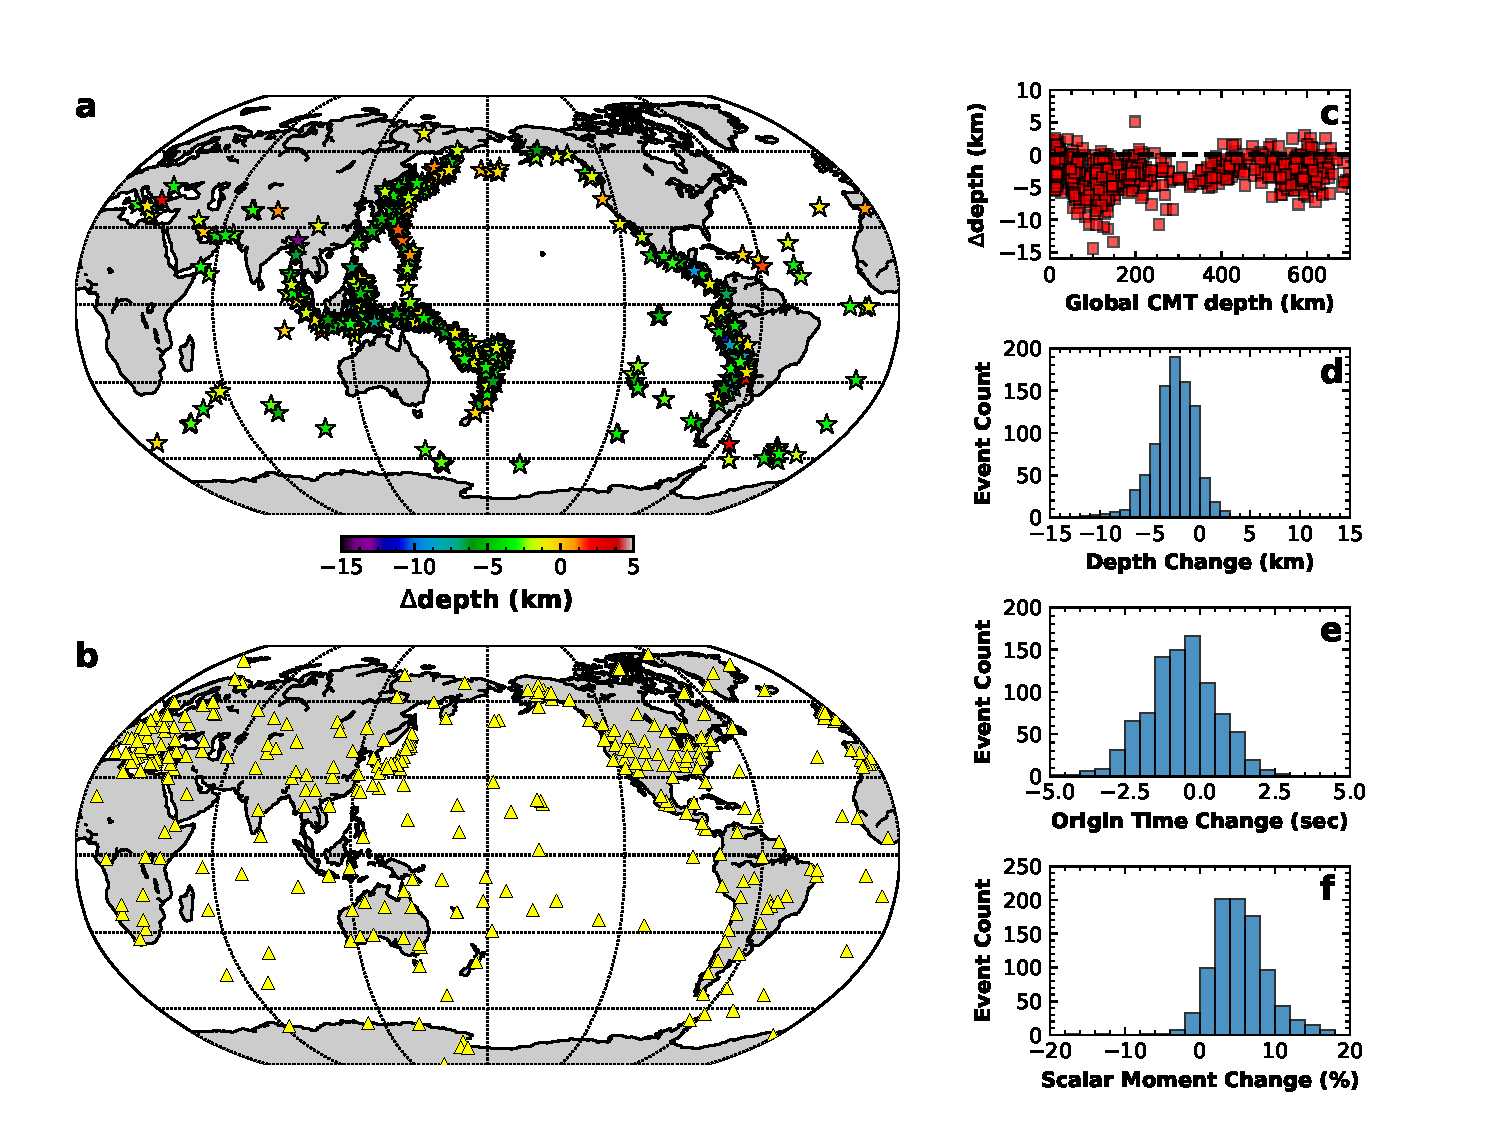
\includegraphics[width=\textwidth]{figures/source_corrections.pdf}
  \caption{\small{Source inversions for 1,040 out of 1,480 events used in the structural inversion. (a) Map view of depth changes. (b) Distribution of seismographic stations used for source inversions. (c) Depth change relative to the original global CMT Catalog depth. (d)--(f) Histograms of depth, origin time, and scalar moment changes relative to the CMT Catalog.
  }}
  \label{fig:source_correction}
\end{figure}

In addition to the 253 earthquakes used for the construction of GLAD-M15, we initially selected 784 additional earthquakes
from the global Centroid-Moment Tensor (CMT) catalog~\citep[e.g.,][]{ekstrom2012global},
resulting in a total number of 1,040 earthquakes.
To ensure a good signal-to-noise ratio on a global scale,
the smallest moment magnitude in the database is set to~5.5 (as in the global CMT catalog),
thereby capturing more deep events,
and, to avoid complications associated with source dimension and directivity,
the largest moment magnitude is set to~7.2.

Before using the 1,040 earthquakes in our structural inversion,
we performed CMT inversions using model GLAD-M15, similar to the 253 events reinverted in the \citet{bozdaug2016global} study using its starting model S362ANI+CRUST2.0,
the results of which are summarized in Fig.~\ref{fig:source_correction}.
To optimize even global coverage,
we used seismographic stations from the  Global Seismic Network (II, IU, IC, US, CU, and GT),
GEOFON~(GE), GEOSCOPE~(G), and several regional networks, such as MedNet~(MN),
the Brazilian Lithospheric Seismic Project~(BL), the Chilean National Seismic Network~(C),
and the Japan Meteorological Agency Seismic Network~(JP) (Fig.~\ref{fig:source_correction}b).
The number of stations used for CMT inversion usually ranges
from~150 to~500 depending on the event dates.

To update the source parameters (six moment tensor components, latitude, longitude and depth) using the starting model to compute the Green's functions for each source parameter,
we used the CMT inversion algorithm of \cite{liu2004spectral}.
This algorithm combines a normalized waveform difference misfit with an envelope difference misfit.
Specifically, the algorithm minimizes the misfit function
\begin{equation}
   \begin{split}
      \Phi =  \sum\limits_{c=1}^{C} \omega_c \sum\limits_{r=1}^{R_c} \omega_{cr}
       \sum\limits_{w=1}^{W_{cr}} \omega_{crw}\,
          & \left\{ \lambda\, \frac
              { \int \big[ d_w(t) - s_w(t - \Delta t) \big]^2 \mathrm{d}t}
              {\int \big[ d_w(t) \big]^2  \mathrm{d}t} \right.
       \\ & \quad \left. \mbox{} + (1 - \lambda)\, \frac
              {\int \big[ e(d_w(t)) - e(s_w(t - \Delta t)) \big]^2 \mathrm{d}t}
              {\int \big[ e(d_w(t)) \big]^2\mathrm{d}t} \right\}
              \quad ,
   \end{split}
\end{equation}
where~$d_w(t)$ denotes data in time window~$w$\,,
and~$s_w(t - \Delta t)$ the corresponding synthetic for model~GLAD-M15.
We allow the synthetics to shift relative to the data by an amount~$\Delta t$
--- effectively a station correction --- determined by cross correlation. We do not invert for the origin times as we minimize the phase misfit due to the station correction, which helps to reduce the nonlinearity of the problem. As we describe later, we take into account the uncertainty in origin times, as well as the scalar moment, by performing an additional grid search at every iteration.
The envelope function is denoted by~$e(\,\cdot\,)$\,,
and the parameter~$\lambda$ determines the balance between fitting waveforms versus fitting envelopes.
The number of measurement categories is denoted by~$C$\,.
Following~\cite{ekstrom2012global},
seismograms were filtered between 50~s and 100~s
to select three-component body-wave windows,
and between 60~s and 100~s to select three-component
surface-wave windows,
resulting in six measurement categories, $c=1,\ldots,C$\,.
To balance their contributions,
each category is weighted by the reciprocal of the number of measurements in that
category, $\omega_c$\,.
The number of windows for a given receiver~$r$ in a given measurement category~$c$ is~$W_{cr}$\,.
Each such window is weighted equally, i.e.,~$\omega_{crw}=1$\,.
The number of receivers that records data in category~$c$ is denoted by~$R_c$\,.
As shown in Fig.~\ref{fig:source_correction}b,
the receivers are unevenly distributed across the globe,
with several dense arrays in the northern hemisphere and poor coverage in the southern hemisphere.
To balance the coverage,
following a strategy articulated by~\cite{Ruanetal2018},
we assign receiver weights~$\omega_{cr}$ based on the expression
\begin{equation}
\omega_{cr}^{-1} = N_c\,\sum_{r'=1}^{R_c} \exp\left[\mbox{}-\left(\frac{\Delta_{rr'}}{\Delta_c}\right)^2\right]
\quad ,
\label{eq:spatial_weights}
\end{equation}
where~$N_c$ is a normalization factor for category~$c$,
and where~$\Delta_{rr'}$ denotes the angular distance between receivers~$r$ and~$r'$\,.
The reference angular distance~$\Delta_c$ for each category~$c$ needs to be chosen such that the condition 
number of the diagonal weighting matrix defined by Eqn.~(\ref{eq:spatial_weights}) is not too large.
The calculation of the weights may be abstracted as: given a distribution of
points on the unit sphere, determine a spatial weighting associated with each point.

The algorithm inverts for the six elements of the moment tensor
and the centroid location~(latitude, longitude, and depth; duration is kept constant).
These source inversions are computationally very expensive,
because for each of the 1,040~events nine full 3D forward simulations are required to obtain the source parameter Fr\'echet derivatives in addition to forward simulation of synthetic seismograms (i.e., 10 forward simulations per event).

Because we allow the synthetics to shift in phase by an amount~$\Delta t$ relative to the data,
the CMT inversion has unreliable sensitivity to the centroid time.
To alleviate this problem,
following~\cite{zhu2012structure},
we perform a subsequent grid search for the centroid time and the scalar moment.
The grid-search calibration involves simple shift and multiply operations on seismograms
and, unlike the CMT inversion, requires minimal simulation time.

Most earthquakes, specifically oceanic ridge events, are shallower after inversion
(Fig.~\ref{fig:source_correction}c),
consistent with our previous experiences~\citep[e.g.,][]{zhu2015seismic,chen2015multiparameter,bozdaug2016global} and with experiments by~\cite{hjorleifsdottir2010effects}. This is partly because the minimum depth of CMT events is fixed to $\sim12$~km, because the sensitivity of source parameters significantly decreases closer to the free surface. 
We observed an average depth change of~$-2.62\pm2.49$~km relative to the global CMT solutions,
an average scalar moment change of~$5.31\pm3.91$\%,
and an average centroid time shift of~$-0.60\pm1.17$~s.
These are relatively minor corrections, mainly due to being conservative in the source inversions to avoid nonlinearities and the not-so-detailed crustal model (an updated version of CRUST2.0 through the 15 iterations performed for GLAD-M15), especially in view of the significant expense of the source inversions.
For this reason, when we added another 440 earthquakes during iteration~22,
thereby bringing the total to~1,480 events,
we only performed a grid search to calibrate the centroid times and scalar moments.

% \subsection{Adaptable Seismic Data Format}
% \label{section:ASDF}

% Conventional seismic data formats, such as SAC, involve one file per time series
% plus related files with instrument response and event information.
% Since every earthquake in the database is typically recorded by thousands of
% instruments, I/O during the preprocessing stage of the adjoint tomography workflow
% quickly cripples the file system. The Adaptable Seismic Data Format
% (ASDF)~\citep[][ \texttt{https://seismic-data.org/}]{krischer2016adaptable}
% was developed with complete reproducibility and fast parallel processing in mind.

% In this context, there are four key issues ASDF resolves.
% \begin{itemize}
%     \item Robustness and stability: the data container is developed and maintained to ensure accuracy of scientific results.
%     \item Data organization: the container is self-describing. Data, including waveform, source, and station information, are organized into well-defined structures.
%     \item Reproducibility: the container enables scientists to keep track of which operations have been performed on the data so that results can be reproduced.
%     \item Efficiency: the format provides easy mechanisms for parallel processing.
% \end{itemize}

% ASDF serves as a self-contained-and-explained data container while taking
% full advantage of parallel computing. In our workflow,
% one ASDF file contains all the information needed for processing one event,
% including the seismic traces, an event information file (in QuakeML format), and station response files (in StationXML format).
% The related Application Programming Interfaces (API)s are carefully designed for easy data extraction and parallel processing.

\section{Adjoint tomography workflow}
\label{section:workflow}

The adjoint tomography workflow is depicted in Fig.~\ref{fig:adjoint_workflow}.
It starts with the selection of earthquakes, as discussed in Section~\ref{section:earthquakes}.
Given the earthquake selection,
observed seismographic data and related response information are acquired.
For a given earthquake,
the corresponding seismograms and related response information are combined in a single ASDF file~\citep{krischer2016adaptable}.
For a given earthquake data set, the conversion to ASDF needs to be performed once and for all.
In the following sections we highlight several important aspects of the workflow.

\begin{figure}
  \centering
  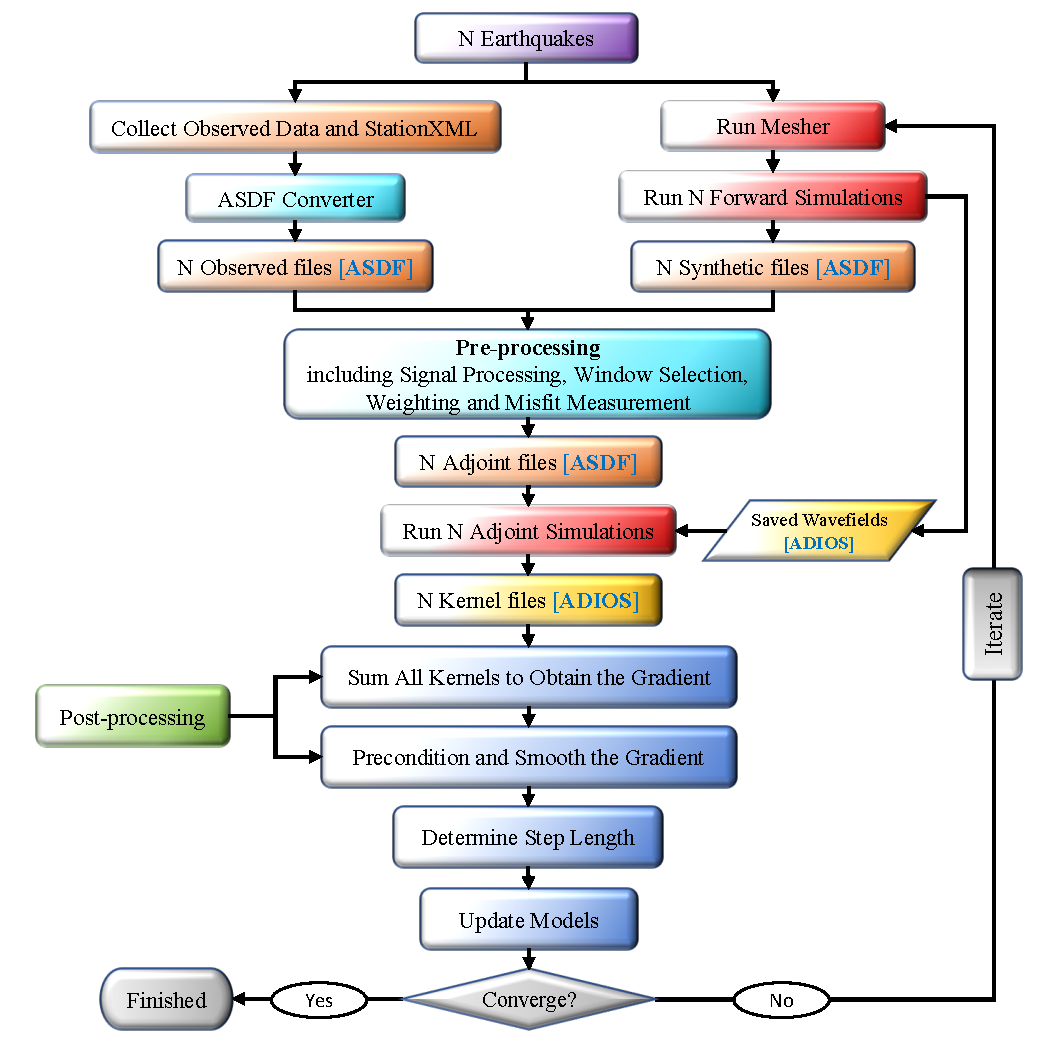
\includegraphics[width=\textwidth]{figures/adjoint_workflow_6.pdf}
  \caption{\small{Adjoint tomography workflow.}}
  \label{fig:adjoint_workflow}
\end{figure}

\subsection{Forward simulations}

The forward simulations are based on the global spectral-element solver
SPECFEM3D\_GLOBE~\citep{KoTr02a,KoTr02a}, and take a CMT solution, a list
of stations, and the current earth model as input.
The solver is GPU accelerated, and the simulations are performed on the Cray ``Titan'' and IBM ``Summit" supercomputers
at the OLCF.

The calculation of Fr\'echet derivatives requires
access to snapshots of the forward wavefield as part of the parsimonious storage
algorithm developed by~\cite{KoXiBoPeSaLiTr16},
with rapid I/O facilitated by ADIOS~\citep{liu2014hello}.
For the current simulation setup,
this requires about 1~TB of storage per earthquake,
so for 1,480 earthquakes this adds up to 1.5~PB.
This temporary volume of data is generated during~$\sim6$~hours of simulations.
Based on our experience, ADIOS is capable of achieving~$\sim120$~GB/s
of sustained I/O on OLCF resources.
Given that typical write speeds for modern hard disks are~$\sim100$~MB/s,
it would be extremely difficult to carry out global adjoint tomography without the ADIOS library.

\subsection{Seismic data processing}

\begin{figure}
  \centering
  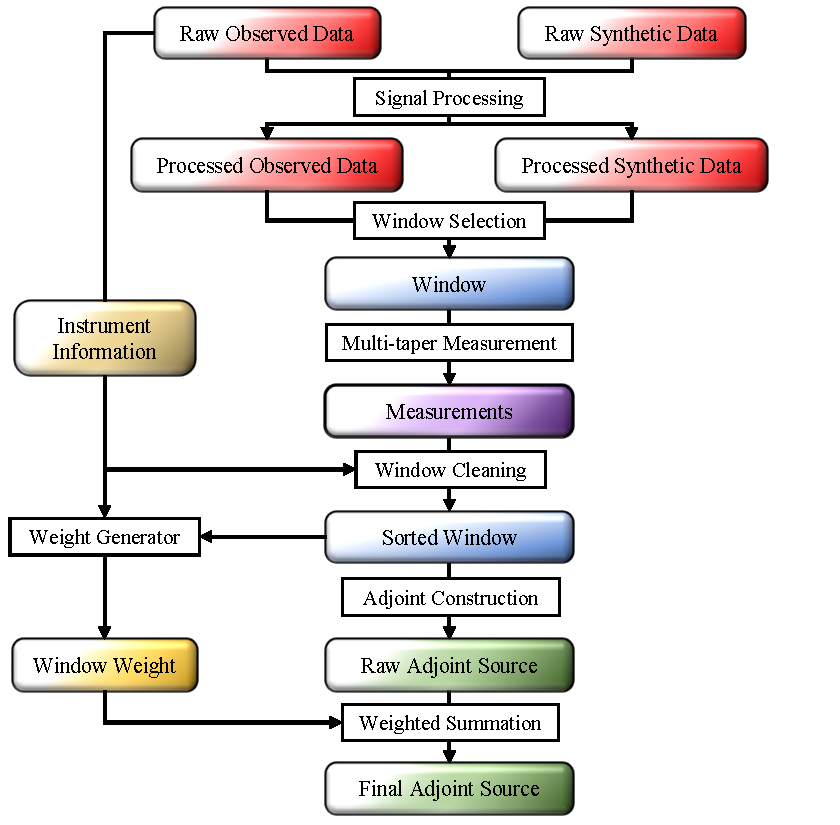
\includegraphics[width=0.8\textwidth]{figures/Preprocess_workflow.pdf}
  \caption{\small{Sub-workflow workflow for preprocessing seismic data.}}
  \label{fig:preprocess_workflow}
\end{figure}

The seismic data preprocessing workflow takes raw observed and synthetic data as input,
and generates adjoint sources for data assimilation as output.
From a computational perspective, the preprocessing workflow consumes only~1\%
of the overall computational requirements.
But from the perspective of the tomographic inversion, this is by far the most
important and tedious stage of the adjoint tomography workflow,
impacting the outcome.

We use millions of seismograms generating tens of millions of measurement windows,
making data selection through human interaction impossible.
The preprocessing workflow automates this task,
most importantly via the time window selection tool FLEXWIN~\citep{maggi2009automated}.

As illustrated in Fig.~\ref{fig:preprocess_workflow}, the preprocessing workflow
includes the following phases.
\begin{enumerate}
  \item Signal processing to remove the instrument response from observed data
    to recover ground displacement using ObsPy~\citep{obspy2010}. Both observed and synthetic data are filtered using the same bandpass, and the horizontal components are rotated to obtain the radial and transverse components of motion.
  \item Window selection on a pair of
    observed and synthetic seismograms. Pyflex (a Python version
    of FLEXWIN by \citet{krischer2015}) is
    used to automatically generate windows where observed and
    synthetic data are sufficiently close to make measurements based on user defined
    criteria.
  \item Cross-correlation traveltime or multi-taper phase measurements in selected windows.
  \item Window sorting and cleaning based on statistical analyses of all measurements to eliminate outliers.
  \item Preliminary adjoint source construction based on the sorted windows.
  \item Calculation and assignment of source and receiver weights~\citep{Ruanetal2018}.
  \item Construction of the final, properly weighted, adjoint sources.
\end{enumerate}

\subsection{Adjoint Simulations}

Collectively,
the adjoint simulations are the most expensive stage of the workflow. 
Adjoint simulations take the adjoint sources as input, and generate Fr\'echet
derivatives of the four model parameters as output.
The computational cost of one adjoint simulation is roughly twice ($\sim25$~min on Titan, less than $10$~min on Summit) that of
a forward simulation, since the forward wavefield is recalculated for convolution with
the adjoint wavefield during the adjoint simulation.
Using this procedure,
both the forward and adjoint wavefields are calculated in forward time,
and attenuation is accurately taken into account in both simulations \citep{KoXiBoPeSaLiTr16}.

\subsection{Postprocessing}

The postprocessing stage of the workflow takes Fr\'echet derivatives as input and
generates a model update as output.
It involves the following steps.
\begin{enumerate}
  \item Summation of the individual Fr\'echet derivatives for each earthquake, called ``event kernels", to obtain the overall gradient of the misfit function. The contribution of each source is weighted to balance
    the uneven distribution of earthquakes~\citep{Ruanetal2018}.
  \item Smoothing of the raw misfit gradient using a 3D Gaussian, which
    serves as a regularization procedure. Instead of using a changing
    smoothing radius based upon the ``kernel density''~\citep{bozdaug2016global},
    we used a fixed value at a given iteration, following~\cite{zhu2012structure}. One can also combine source-receiver weighting with the multi-stage smoothing strategy to highlight structure underneath densely covered regions, as in~\citet{bozdaug2016global}.
  \item Preconditioning of the smoothed gradient based on a technique proposed by~\cite{luo2013strategies}.
  \item Line search in the direction of the negative gradient to determine the magnitude of the model update.
  The search direction is determined using a nonlinear conjugate gradient method (iterations 16--21) or a Limited-memory Broyden- Fletcher-Goldfarb-Shanno (L-BFGS) quasi-Newton method (iterations 22--25)~\citep{wright1999numerical}.
  We used a subset of 160 earthquakes to conduct the line search and determine the step length. One can also determine the step length using the Wolf criteria, which are commonly used in exploration studies \cyan{reference}. We prefer to perform the line search to be able to keep track of the evolution of the misfit in every measurement category.
\end{enumerate}

\subsection{Workflow management}

There are more than ten stages in the adjoint tomography workflow,
and each stage involves thousands of small repeated tasks.
For every model iteration,
we performed up to 1,480 forward and adjoint simulations, each involving hundreds of
compute cores and graphics cards, as well as heavy I/O.
The workflow is prone to human error and hardware failure, making it fragile~~\citep{Lefebvre2018}.
For these reasons, we hardened the workflow by taking advantage of modern
workflow management software.
We have selected EnTK as our
workflow management engine~\citep{EnTK2017}, and developed complementary seismic tomography
workflow tools.
The workflow engine can automatically detected job failures both from the
HPC system and via user-defined functions. This enables us to keep track of
all tasks and semi-automatically resubmit jobs if necessary.
Given that most HPC system time is spent waiting in the job queue, automatic
failure detection and relaunching greatly shortens the overall time to solution.

% \subsection{Misfit assessment}
% \label{section:Misfit assessment}

% \subsection{Histogram comparisons}
% \label{section:Histogram comparisons}

% Fig.~\ref{fig:PS_phase_hist} shows histograms of 17--40~s P-wave traveltime anomalies on the vertical and radial components, and 17-40~s S-wave traveltime anomalies on the transverse component.
% Both P and S waves exhibit consistent reductions in terms of both mean and variance. 

% \begin{figure}
%   \centering
%   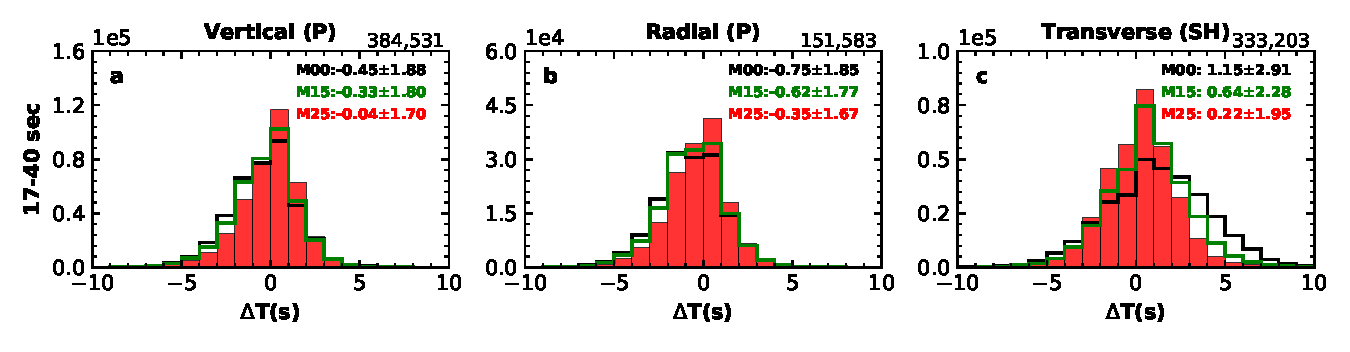
\includegraphics[width=\textwidth]{figures/dt_histogram_phase.pdf}
%   \caption{\small{Histograms of 17--40~s traveltime anomalies of P (vertical and radial), and SH (Transverse) arrivals for models S362ANI combined with CRUST2.0 (M00, Black), GLAD-M15 (M15, Green), and GLAD-M25 (M25, Red).
%   }}
%   \label{fig:PS_phase_hist}
% \end{figure}

% Fig.~\ref{fig:amp_hist} shows histograms of the amplitude
% measurements for all twelve measurement categories,
% which were not used in the current inversion.
% Despite this,
% we observe modest reductions in all standard deviations of the histograms.
% The histograms are nicely centered, indicating that the moment magnitudes are
% suitably selected, because the scalar moment affects all measurement categories equally.
% In the next phase of our ongoing inversion we plan to begin assimilating amplitude measurements while simultaneously adding shear attenuation as a new model parameter.

% \begin{figure}
%   \centering
%   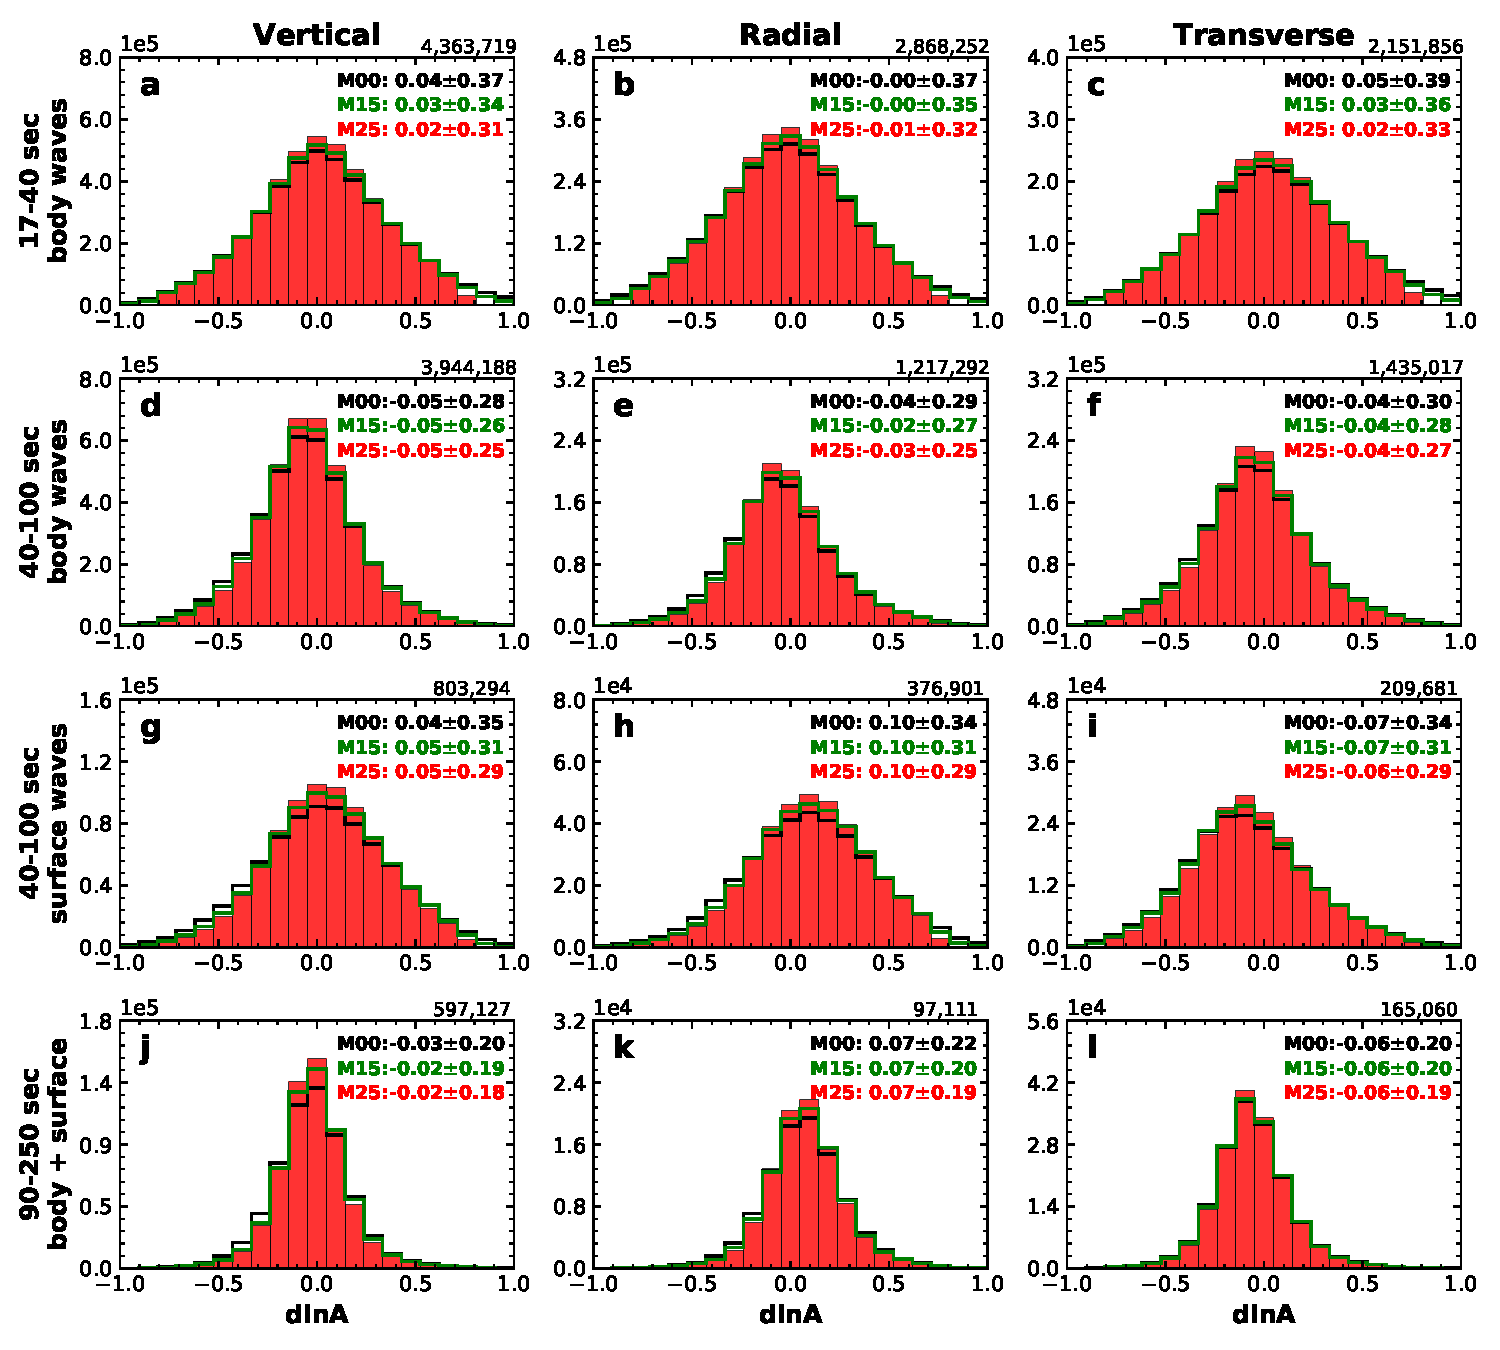
\includegraphics[width=\textwidth]{figures/dlna_histogram.pdf}
%   \caption{\small{Same as Fig.~\ref{fig:phase_hist} except for amplitude measurements. These measurements are currently not used in the inversion.}}
%   \label{fig:amp_hist}
% \end{figure}

\section{Point Spread Function tests}

This section summarizes the complete Point Spread Function (PSF) tests conducted as part of this study, including the tradeoff between parameters.
Figs.~\ref{fig:psf_yellowstone}--\ref{fig:psf_su} show the results of PSF tests underneath Yellowstone, Easter Island, Afar, and Sumatra.
Each figure shows the original Gaussian perturbation in vertically polarized shear wavespeed, $\mathsf{\Delta}\mathsf{m}$\,, in map view and cross section, as well as the action of the Hessian on this model perturbation, $\mathsf{H}\mathsf{\Delta}\mathsf{m}$\,.

We used different sized Gaussian perturbations in the PSF tests, from 160~to~400~km in diameter depending on the kernel coverage of the selected regions, both in the upper and lower mantle. Although we observe some smearing effects, the Gaussian anomalies are overall well-recovered. As expected, PSF tests are most successful in North America, where we have the best coverage, thanks to USArray. However, it is also encouraging to see good recovery in the lower mantle to assess the resolution of lower-mantle plumes. We observe limited smearing onto other parameters, e.g., we observe a slight tradeoff in radial anisotropy in the upper mantle for the tests performed underneath North America.

\begin{figure}
  \centering
  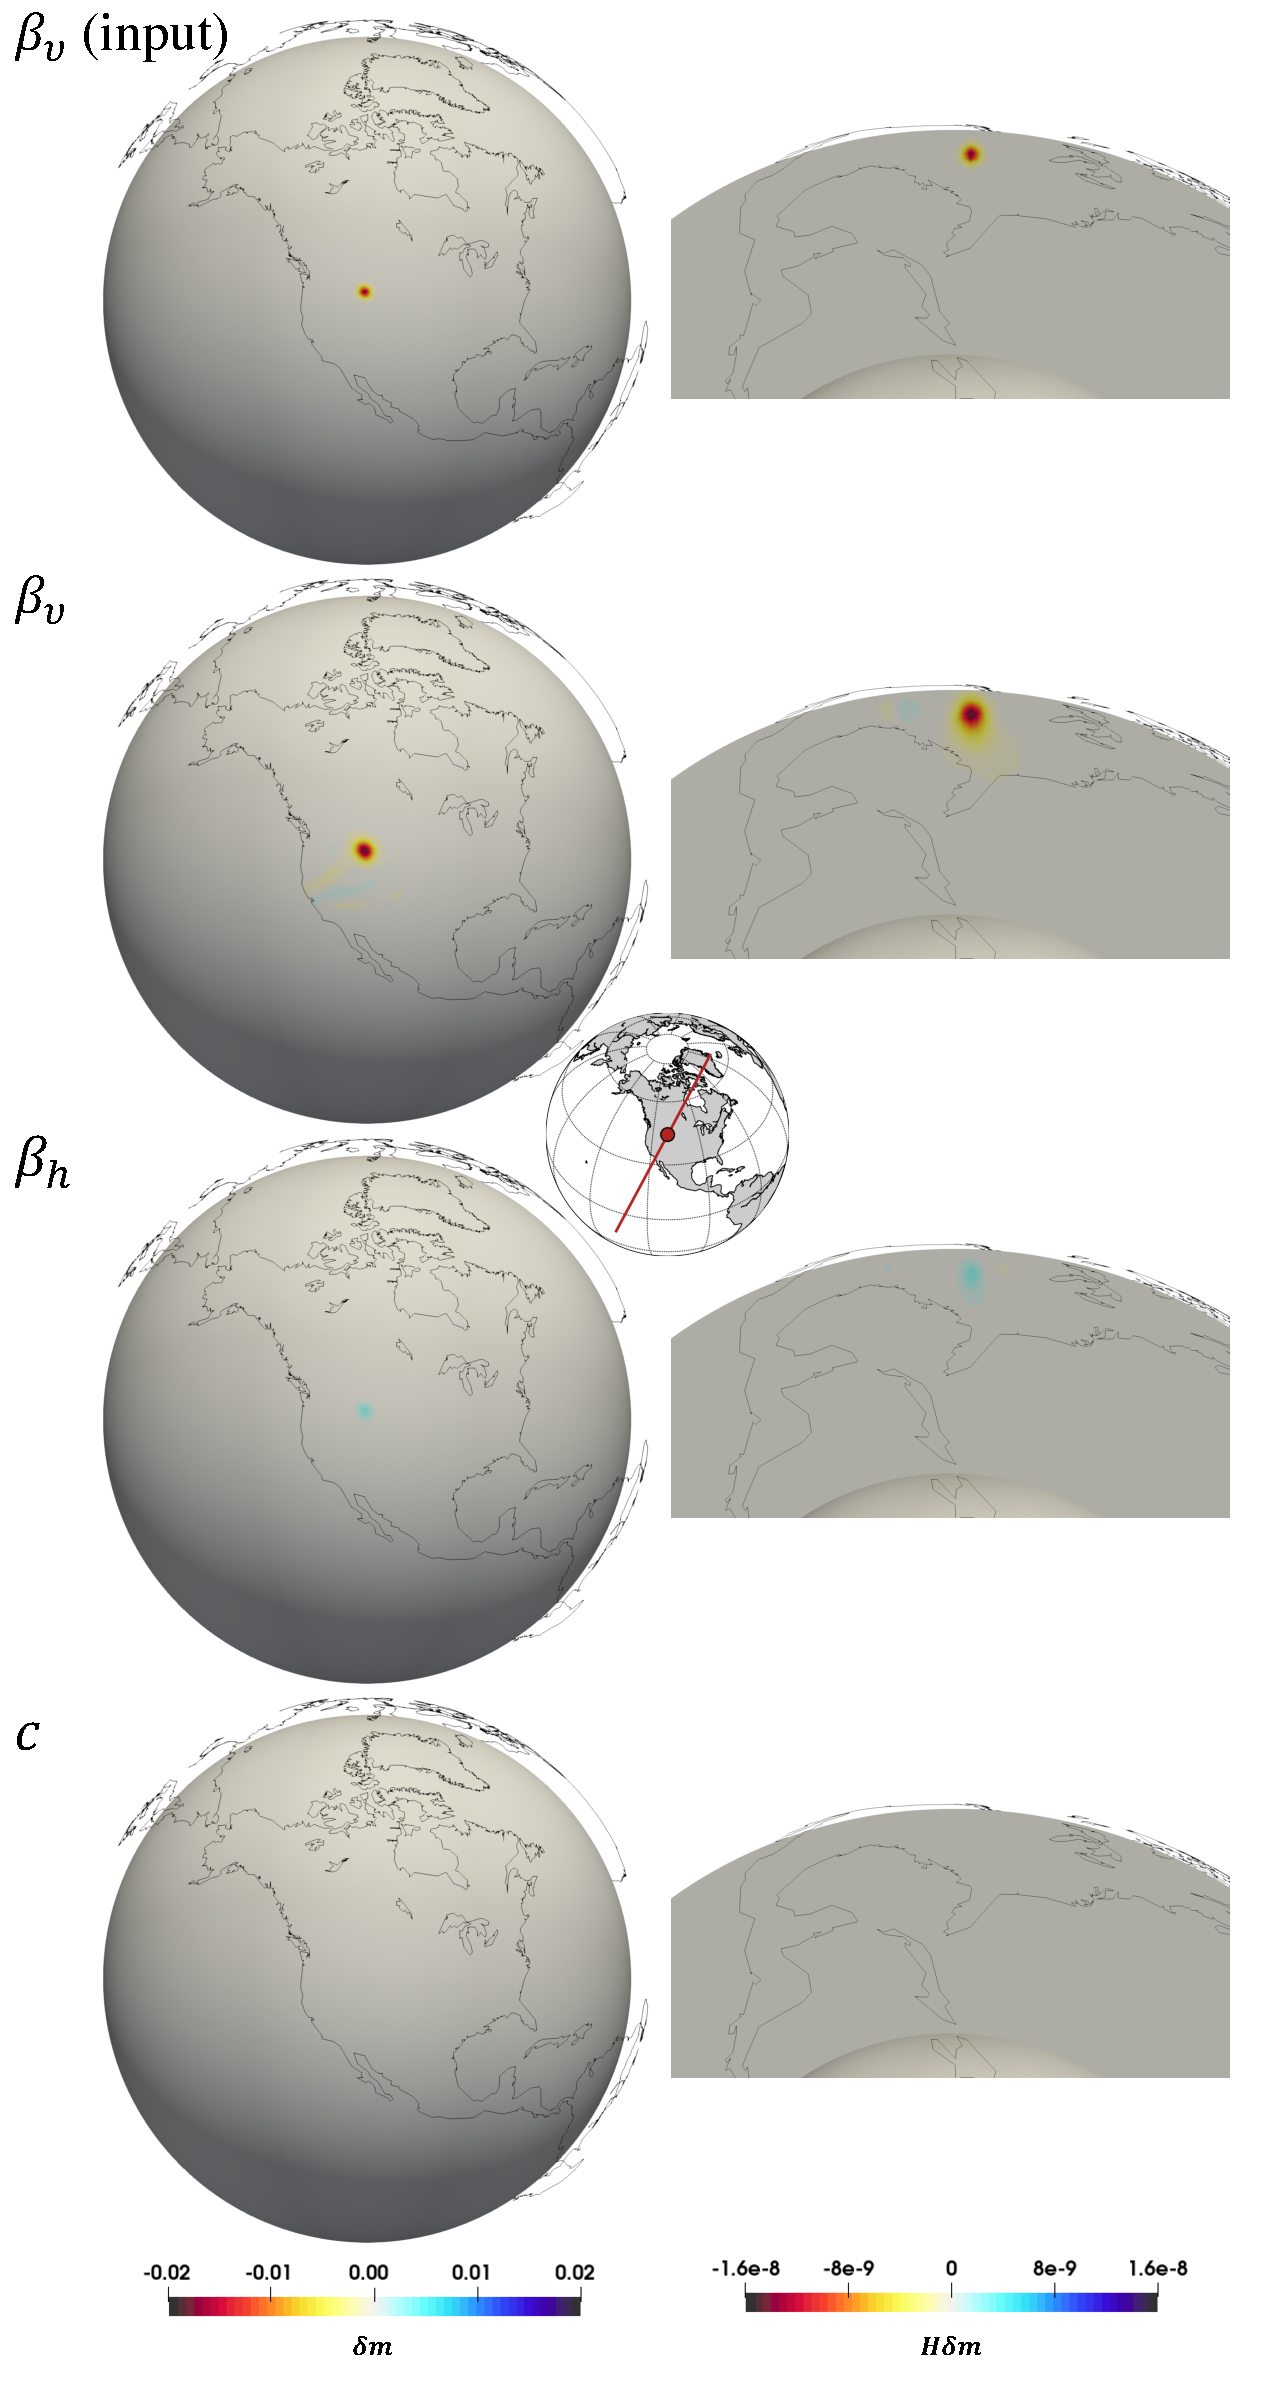
\includegraphics[width=0.65\textwidth]{figures/psf/yellowstone.pdf}
  \caption{\small{PSF test for Yellowstone.
  A 100~km diameter negative Gaussian anomaly is placed at a depth of 300~km beneath Yellowstone.
  Top row: Map view (Left) and cross section (Right) through a Gaussian perturbation in~$\beta_\mathrm{V}$.
  Second row: Map view (Left) and cross section (Right) through the recovered perturbation in~$\beta_\mathrm{V}$.
  Third row: Map view (Left) and cross section (Right) through the recovered perturbation in~$\beta_\mathrm{H}$.
  Bottom row: Map view (Left) and cross section (Right) through the recovered perturbation in the bulk sound speed~$c$. We conclude that there is little tradeoff between~$\beta_\mathrm{V}$ and~$\beta_\mathrm{H}$ and ~$c$.
  }}
  \label{fig:psf_yellowstone}
\end{figure}

\begin{figure}
  \centering
  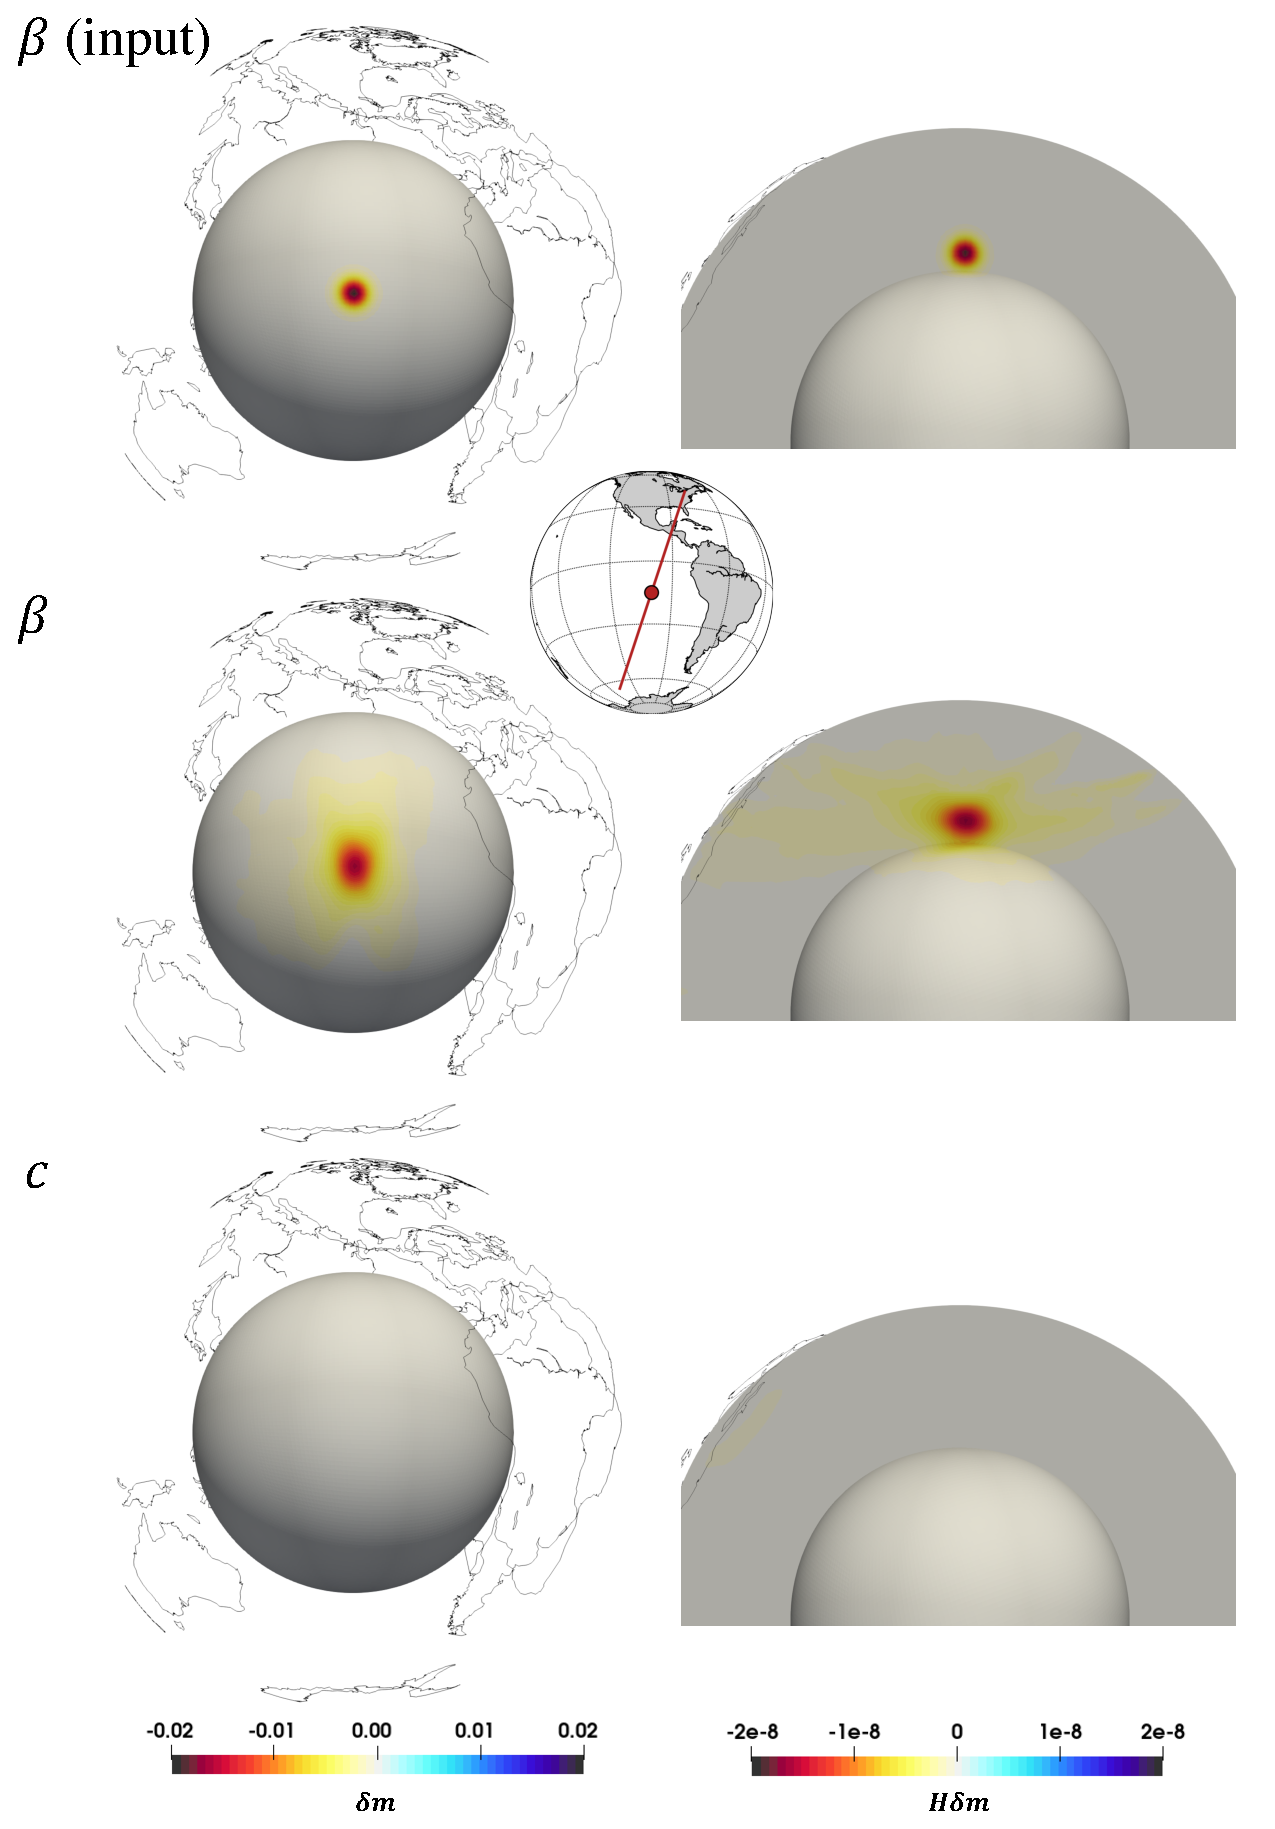
\includegraphics[width=0.65\textwidth]{figures/psf/easter.pdf}
  \caption{\small{PSF test for Easter Island.
  A 300~km diameter negative Gaussian anomaly is placed at a depth of 2,500~km beneath Easter Island.
  Top row: Map view (Left) and cross section (Right) through a Gaussian perturbation in~$\beta_\mathrm{V}$.
  Second row: Map view (Left) and cross section (Right) through the recovered perturbation in~$\beta_\mathrm{V}$.
  Third row: Map view (Left) and cross section (Right) through the recovered perturbation in~$\beta_\mathrm{H}$.
  Bottom row: Map view (Left) and cross section (Right) through the recovered perturbation in the bulk sound speed~$c$. We conclude that there is little tradeoff between~$\beta_\mathrm{V}$ and~$\beta_\mathrm{H}$ and ~$c$.  A 75~km diameter positive Gaussian anomaly is placed at a depth of 150~km beneath Yellowstone.
  Top row: Map view (Left) and cross section (Right) through a Gaussian perturbation in~$\beta_\mathrm{V}$.
  Second row: Map view (Left) and cross section (Right) through the recovered perturbation in~$\beta_\mathrm{V}$.
  Third row: Map view (Left) and cross section (Right) through the recovered perturbation in~$\beta_\mathrm{H}$.
  Bottom row: Map view (Left) and cross section (Right) through the recovered perturbation in the bulk sound speed~$c$. We conclude that there is little tradeoff between~$\beta_\mathrm{V}$ and~$\beta_\mathrm{H}$ and ~$c$.}}
  \label{fig:psf_easter}
\end{figure}

\begin{figure}
  \centering
  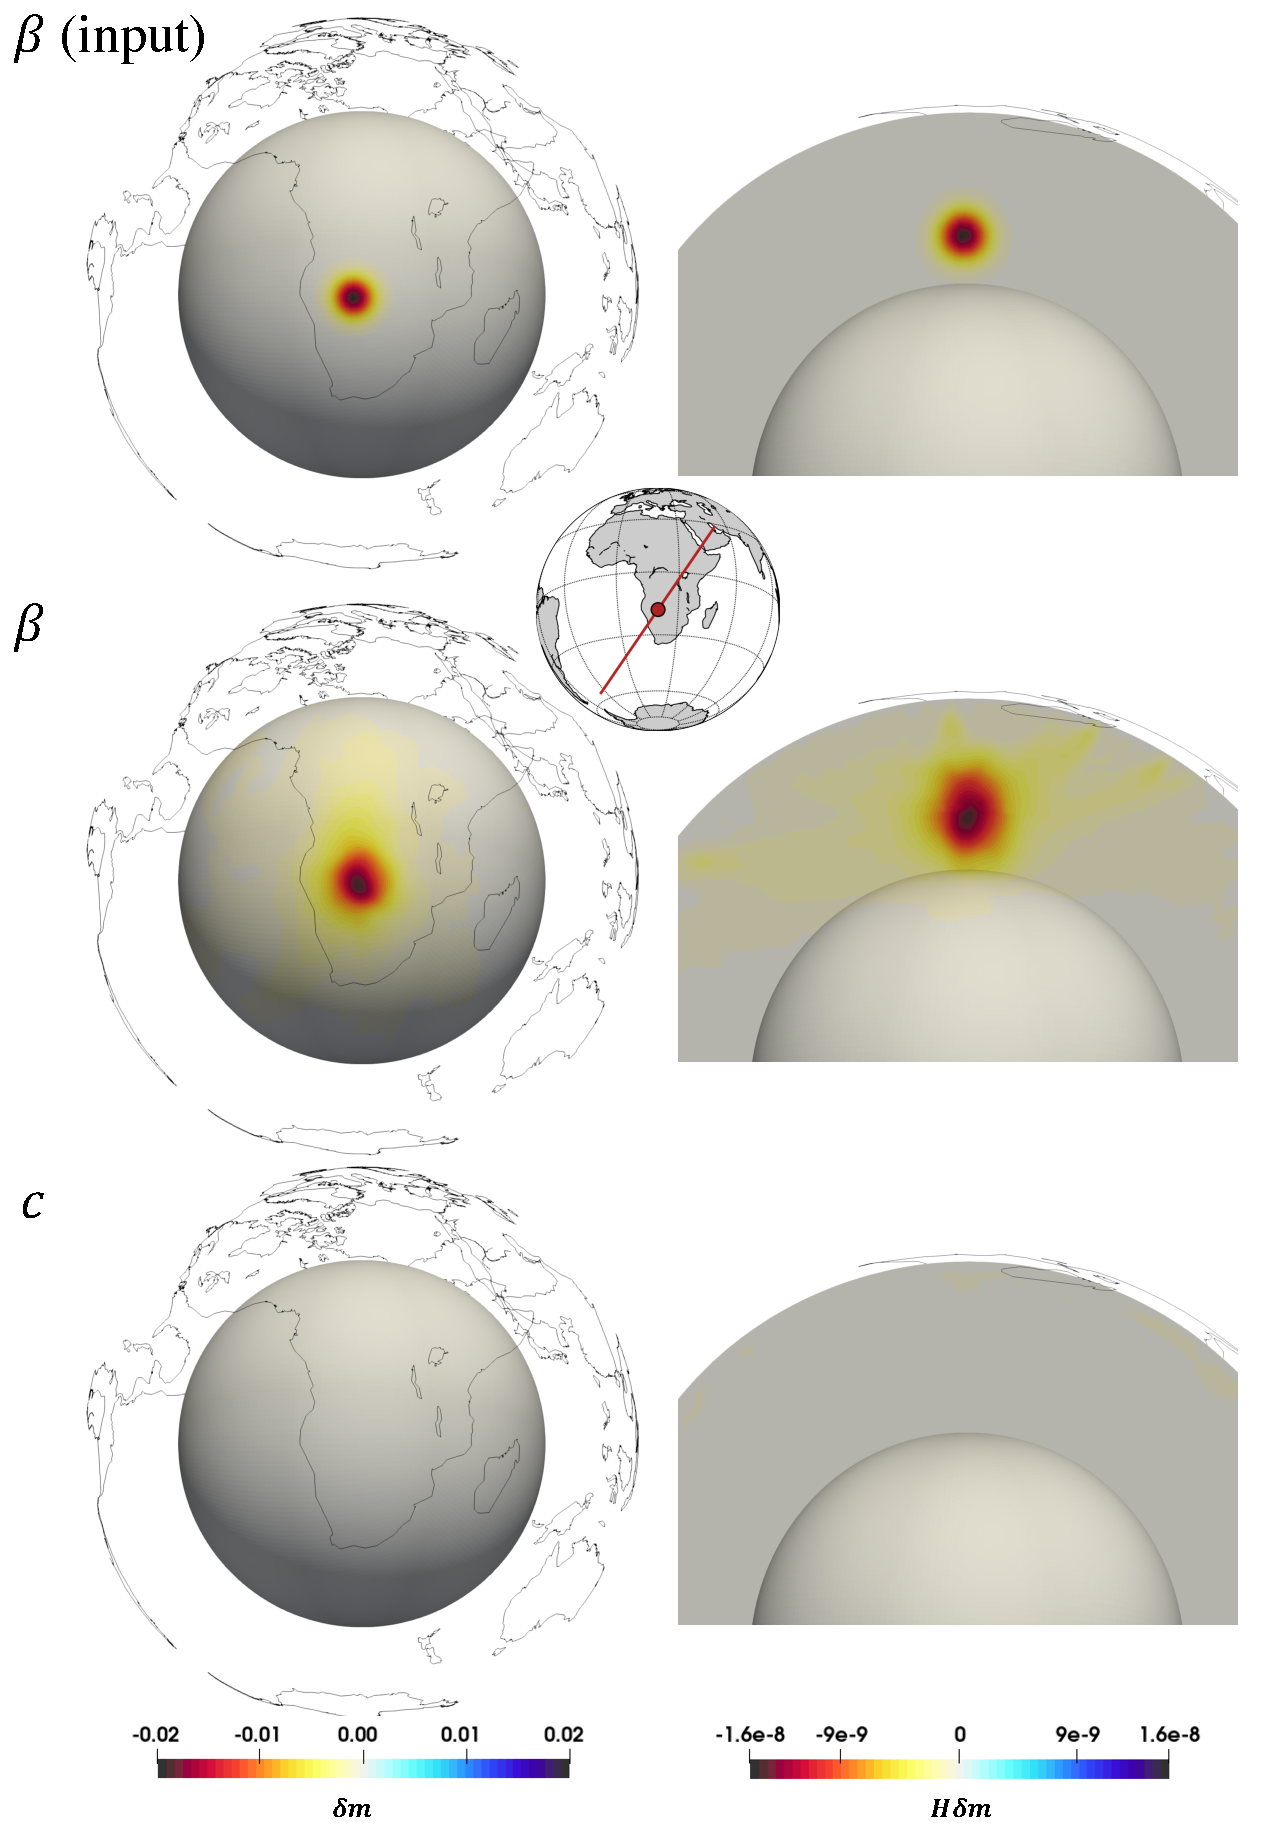
\includegraphics[width=0.65\textwidth]{figures/psf/afar.pdf}
  \caption{\small{PSF test for Afar.
    A 400~km diameter negative Gaussian anomaly is placed at a depth of 2,000~km beneath Afar.
  Top row: Map view (Left) and cross section (Right) through a Gaussian perturbation in~$\beta_\mathrm{V}$.
  Second row: Map view (Left) and cross section (Right) through the recovered perturbation in~$\beta_\mathrm{V}$.
  Third row: Map view (Left) and cross section (Right) through the recovered perturbation in~$\beta_\mathrm{H}$.
  Bottom row: Map view (Left) and cross section (Right) through the recovered perturbation in the bulk sound speed~$c$. We conclude that there is little tradeoff between~$\beta_\mathrm{V}$ and~$\beta_\mathrm{H}$ and ~$c$.
  }}
  \label{fig:psf_afar}
\end{figure}

\begin{figure}
  \centering
  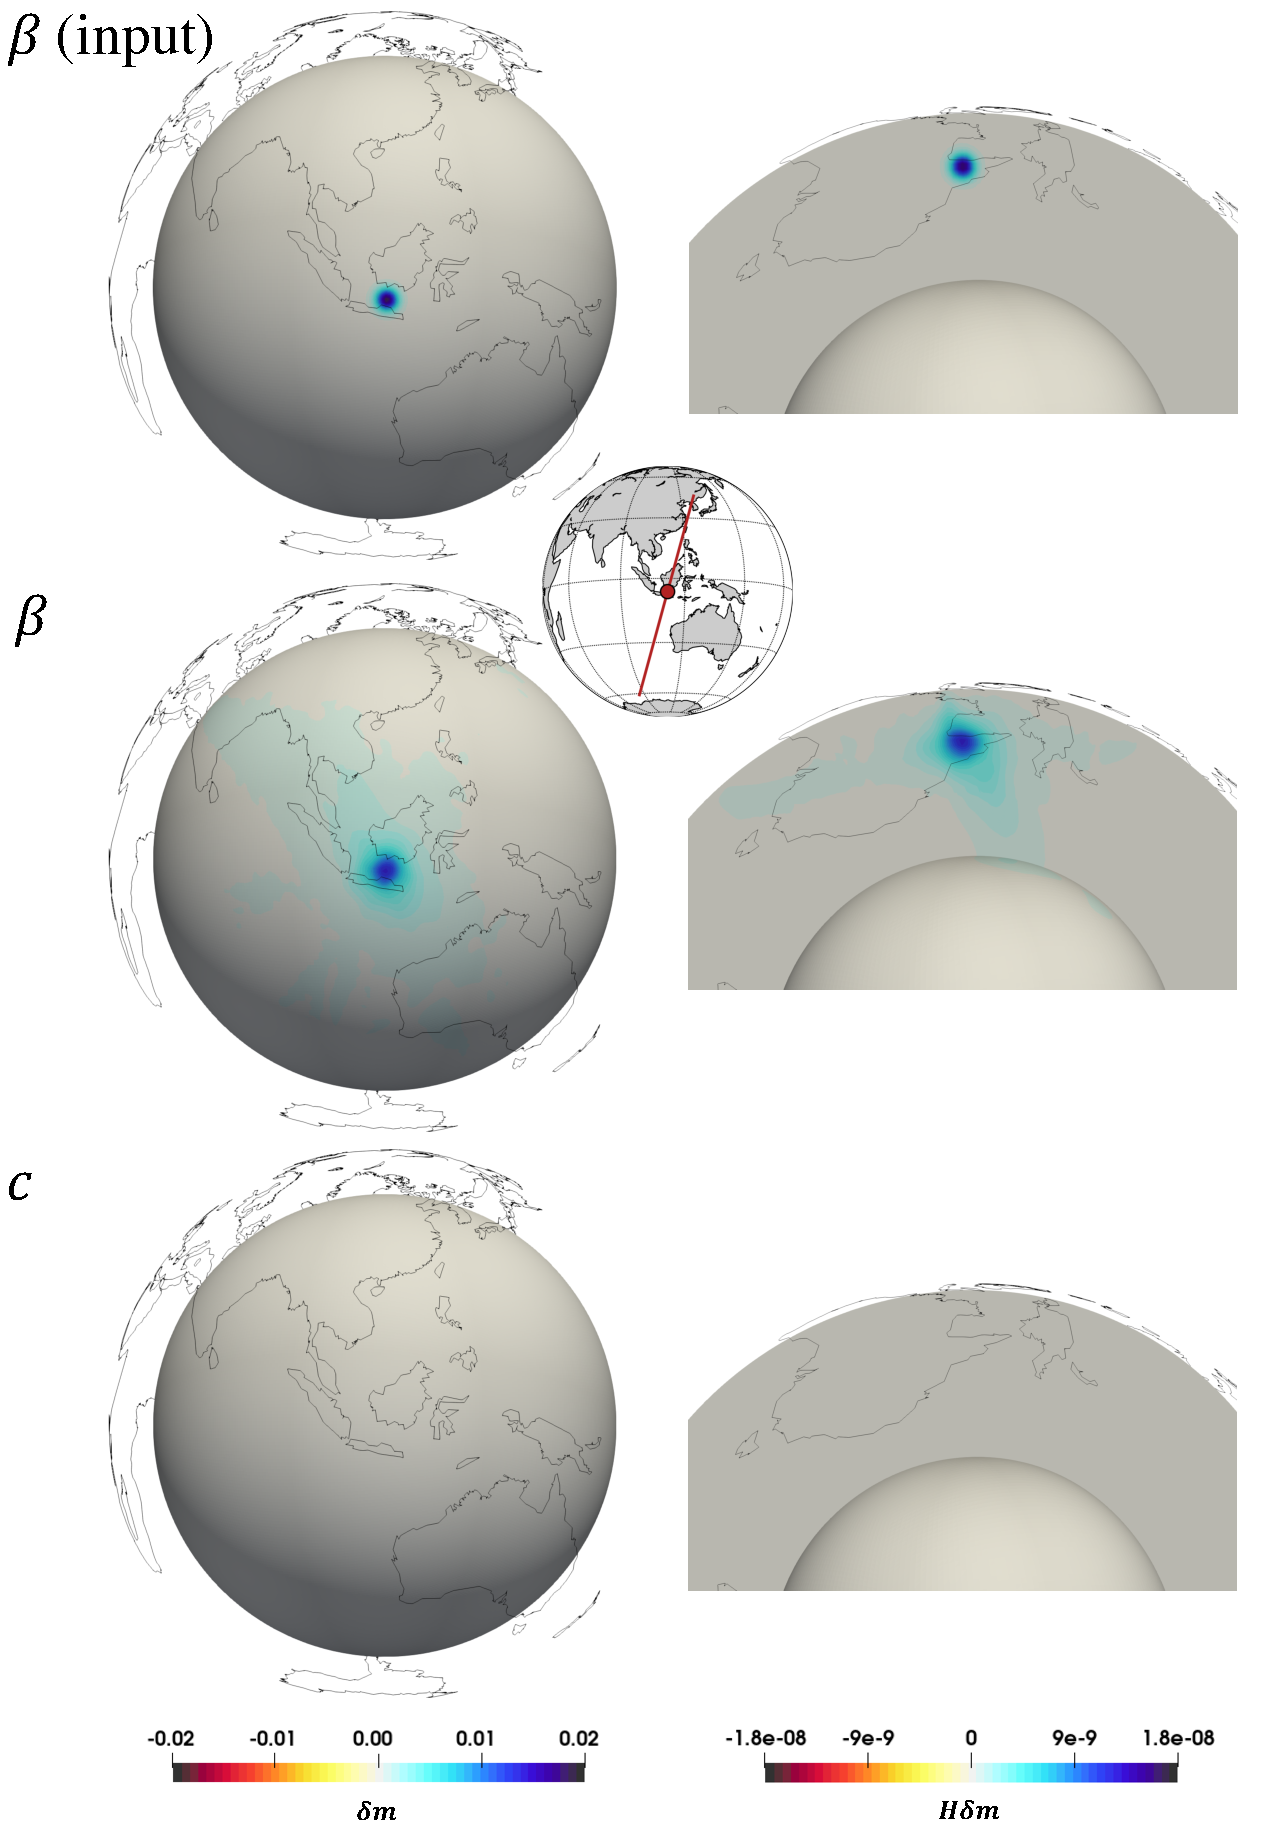
\includegraphics[width=0.65\textwidth]{figures/psf/su.pdf}
  \caption{\small{PSF test for Sumatra.
    A 200~km diameter positive Gaussian anomaly is placed at a depth of 900~km beneath Sumatra.
  Top row: Map view (Left) and cross section (Right) through a Gaussian perturbation in~$\beta_\mathrm{V}$.
  Second row: Map view (Left) and cross section (Right) through the recovered perturbation in~$\beta_\mathrm{V}$.
  Third row: Map view (Left) and cross section (Right) through the recovered perturbation in~$\beta_\mathrm{H}$.
  Bottom row: Map view (Left) and cross section (Right) through the recovered perturbation in the bulk sound speed~$c$. We conclude that there is little tradeoff between~$\beta_\mathrm{V}$ and~$\beta_\mathrm{H}$ and ~$c$.
  }}
  \label{fig:psf_su}
\end{figure}

\begin{figure}
  \centering
  \includegraphics[width=0.65\textwidth]{figures/psf/usa_mid.pdf}
  \caption{\small{PSF test for the middle of the United States.
    A 160~km diameter negative Gaussian anomaly is placed at a depth of 500~km beneath the middle of the US.
  Top row: Map view (Left) and cross section (Right) through a Gaussian perturbation in~$\beta_\mathrm{V}$.
  Second row: Map view (Left) and cross section (Right) through the recovered perturbation in~$\beta_\mathrm{V}$.
  Third row: Map view (Left) and cross section (Right) through the recovered perturbation in~$\beta_\mathrm{H}$.
  Bottom row: Map view (Left) and cross section (Right) through the recovered perturbation in the bulk sound speed~$c$. We conclude that there is little tradeoff between~$\beta_\mathrm{V}$ and~$\beta_\mathrm{H}$ and ~$c$.
  }}
  \label{fig:psf_usa_mid}
\end{figure}


\begin{figure}
  \centering
  \includegraphics[width=0.65\textwidth]{figures/psf/usa_east.pdf}
  \caption{\small{PSF test underneath the eastern United States.
    A 250~km diameter positive Gaussian anomaly is placed at a depth of 1500~km beneath the eastern US.
  Top row: Map view (Left) and cross section (Right) through a Gaussian perturbation in~$\beta_\mathrm{V}$.
  Second row: Map view (Left) and cross section (Right) through the recovered perturbation in~$\beta_\mathrm{V}$.
  Third row: Map view (Left) and cross section (Right) through the recovered perturbation in~$\beta_\mathrm{H}$.
  Bottom row: Map view (Left) and cross section (Right) through the recovered perturbation in the bulk sound speed~$c$. We conclude that there is little tradeoff between~$\beta_\mathrm{V}$ and~$\beta_\mathrm{H}$ and ~$c$.
  }}
  \label{fig:psf_usa_east}
\end{figure}


\section{Model GLAD-M25}
\label{section:model}

In this section we discuss model GLAD-M25 in some detail.
We begin with a global overview of the model, before concentrating on
specific geographical regions.

\subsection{More Comparisons with GLAD-M15}

In addition to section~7.1, we provide more detailed comparisons with GLAD-M15. Fig.~\ref{fig:m15_hotspot} shows the comparisons of $V_{sv}$ perturbations in the plumes and Fig.~\ref{fig:m15_subudction} shows comparisons n the subduction areas. In both comparison figures, GLAD-M25 shows significant enhancement and emerging features compared to GLAD-M15.

\begin{figure}
  \centering
  \includegraphics[width=0.75\textwidth]{figures/compare_M15/hotspot.pdf}
  \caption{\small{Vertical cross sections for various plumes and hotspots for model GLAD-M15($V_\textrm{sv}$, left column) and GLAD-M25($V_\textrm{sv}$; right column).
  The map in the middle shows the cross section with color-coded red, green, and white dots for geographical reference; hotspots are denoted by red triangles.
  The dashed black semicircles in the cross sections denote depths of 410~km, 660~km, and 1000~km.
  (a) Afar; (b) Canary (left) and Hoggar (right); (c) Easter (left) and Galapagos (right); (d) Samoa; (e) Tahiti (middle) and Macdonald (right); (f) Iceland.
  }}
  \label{fig:m15_hotspot}
\end{figure}

\begin{figure}
  \centering
  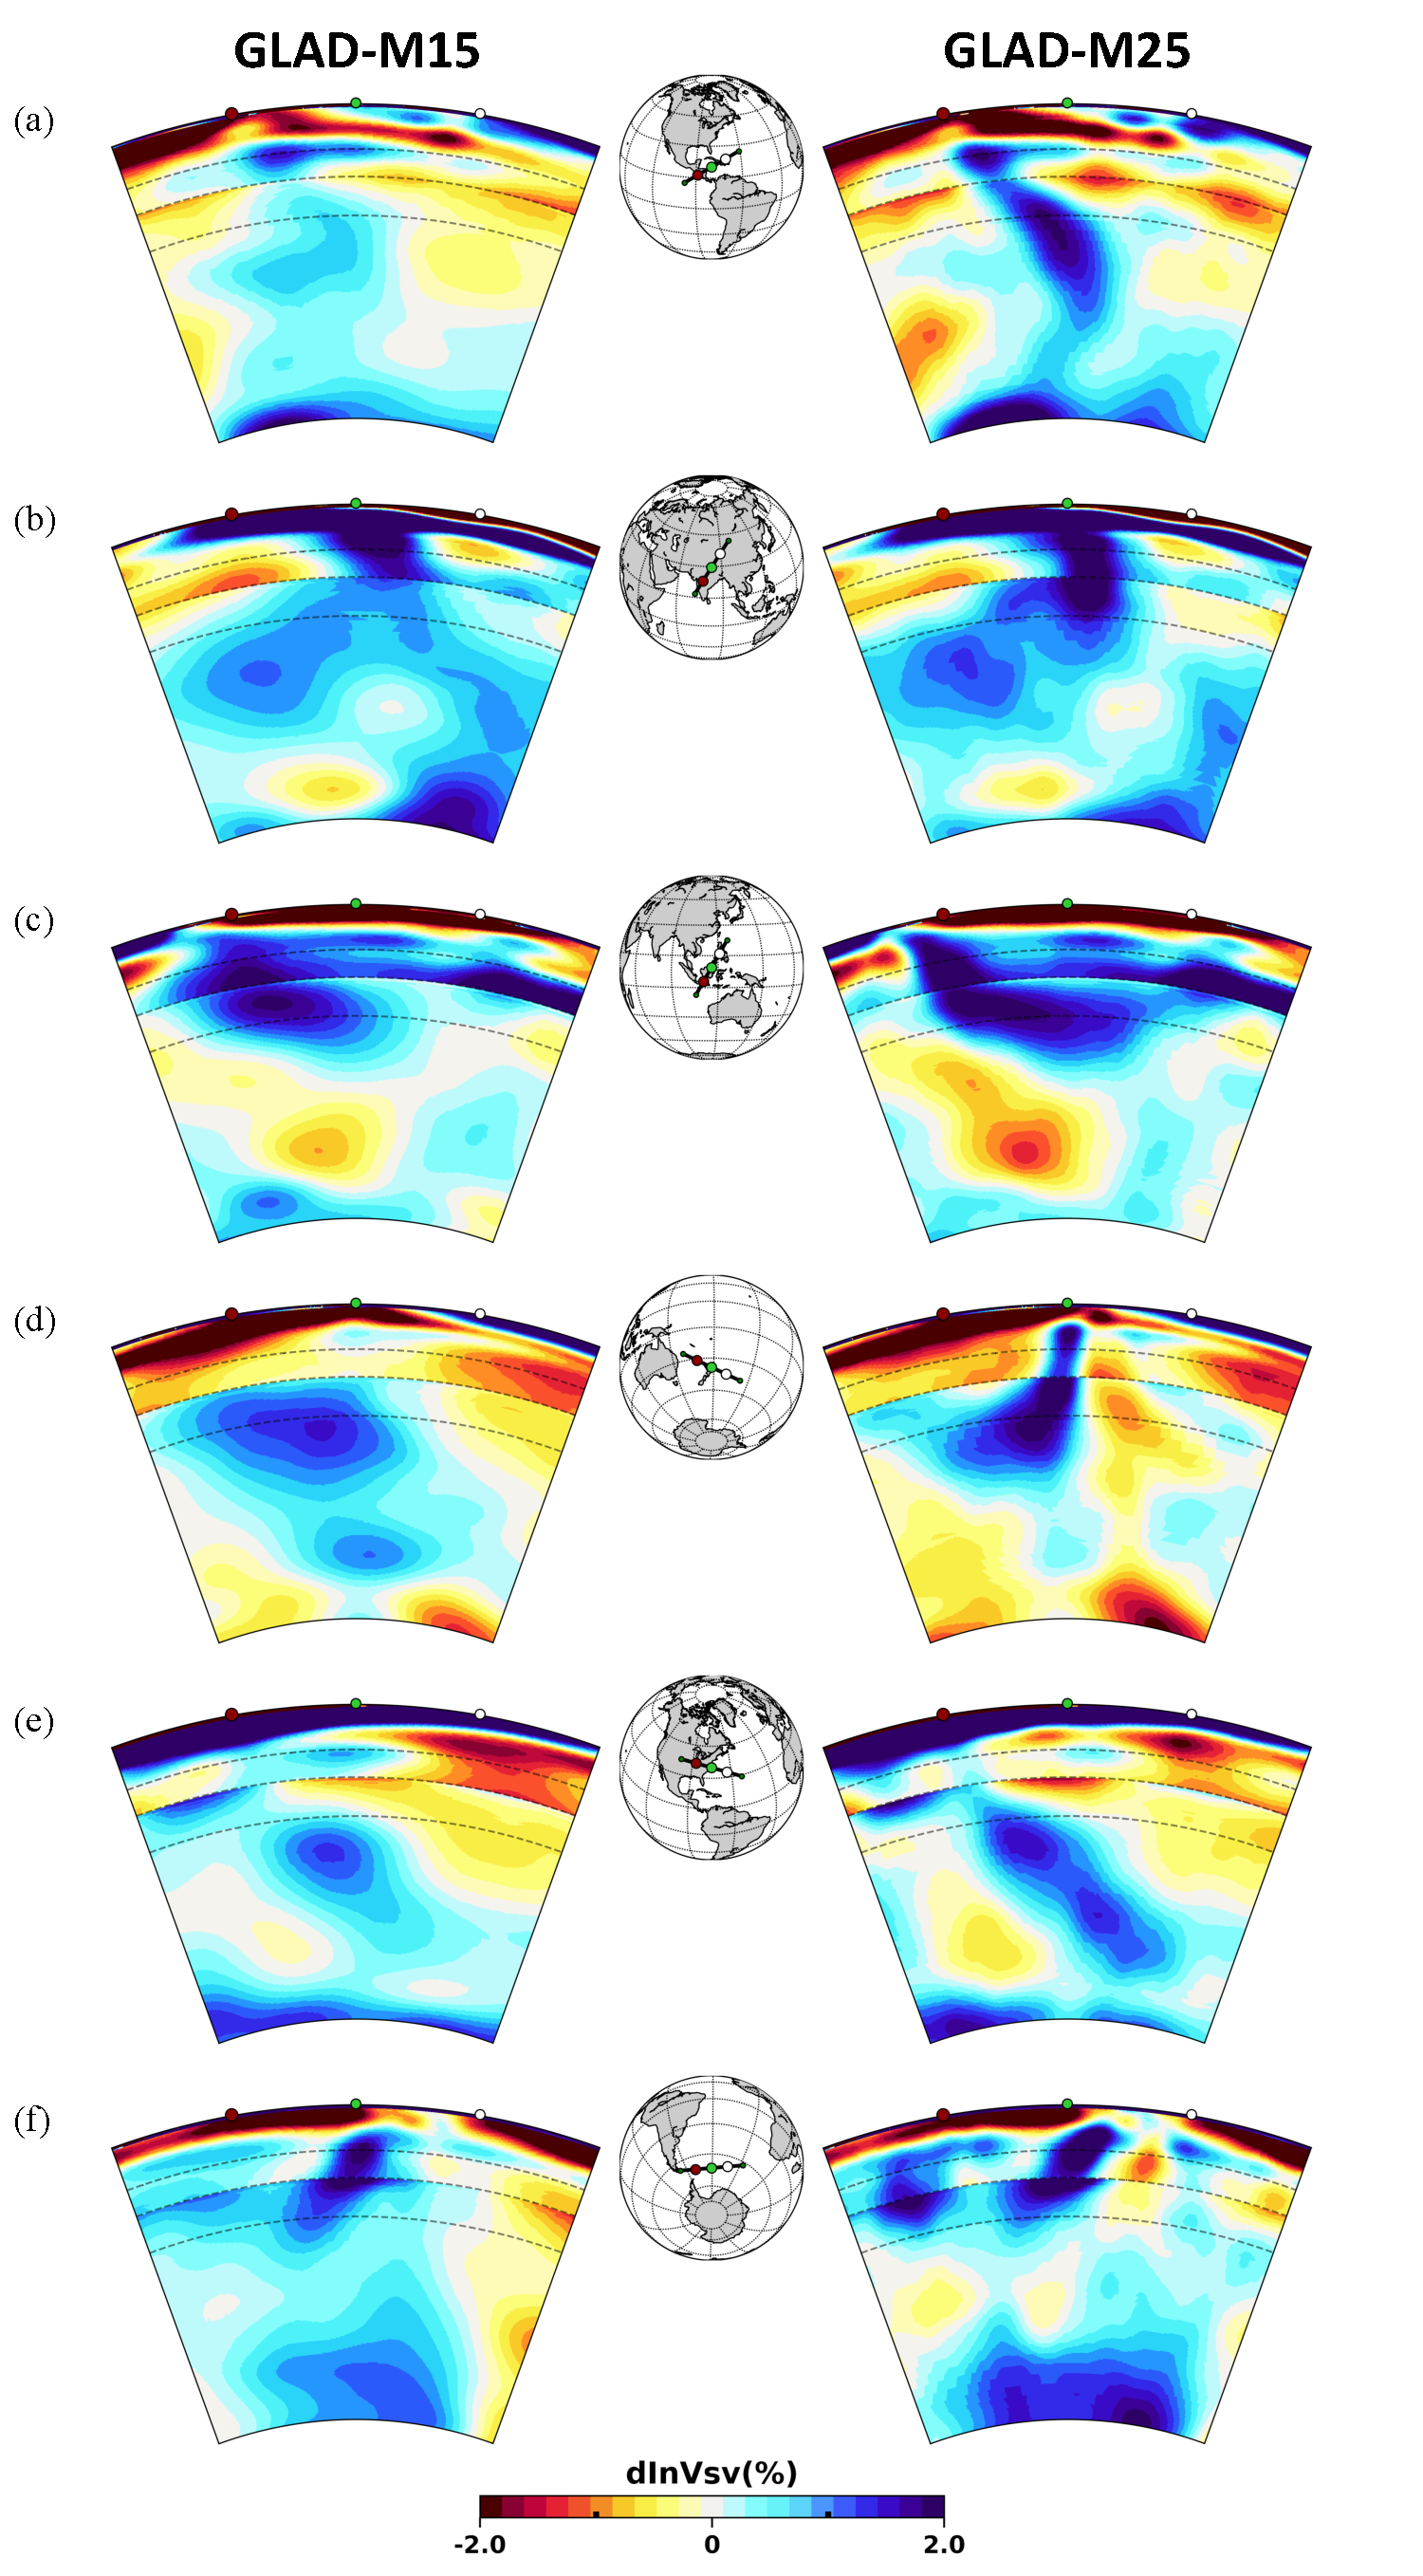
\includegraphics[width=0.7\textwidth]{figures/compare_M15/subduction.pdf}
  \caption{\small{ Vertical cross sections for various subduction regions, same as Fig.~\ref{fig:m15_hotspot}.
  (a) Cocos; (b) India; (c) Sumatra; (d) Fiji-Tonga; (e) Farallon; (f) Scotia. }}
  \label{fig:m15_subduction}
\end{figure}


\subsection{Global structure}

\begin{figure}
  \centering
  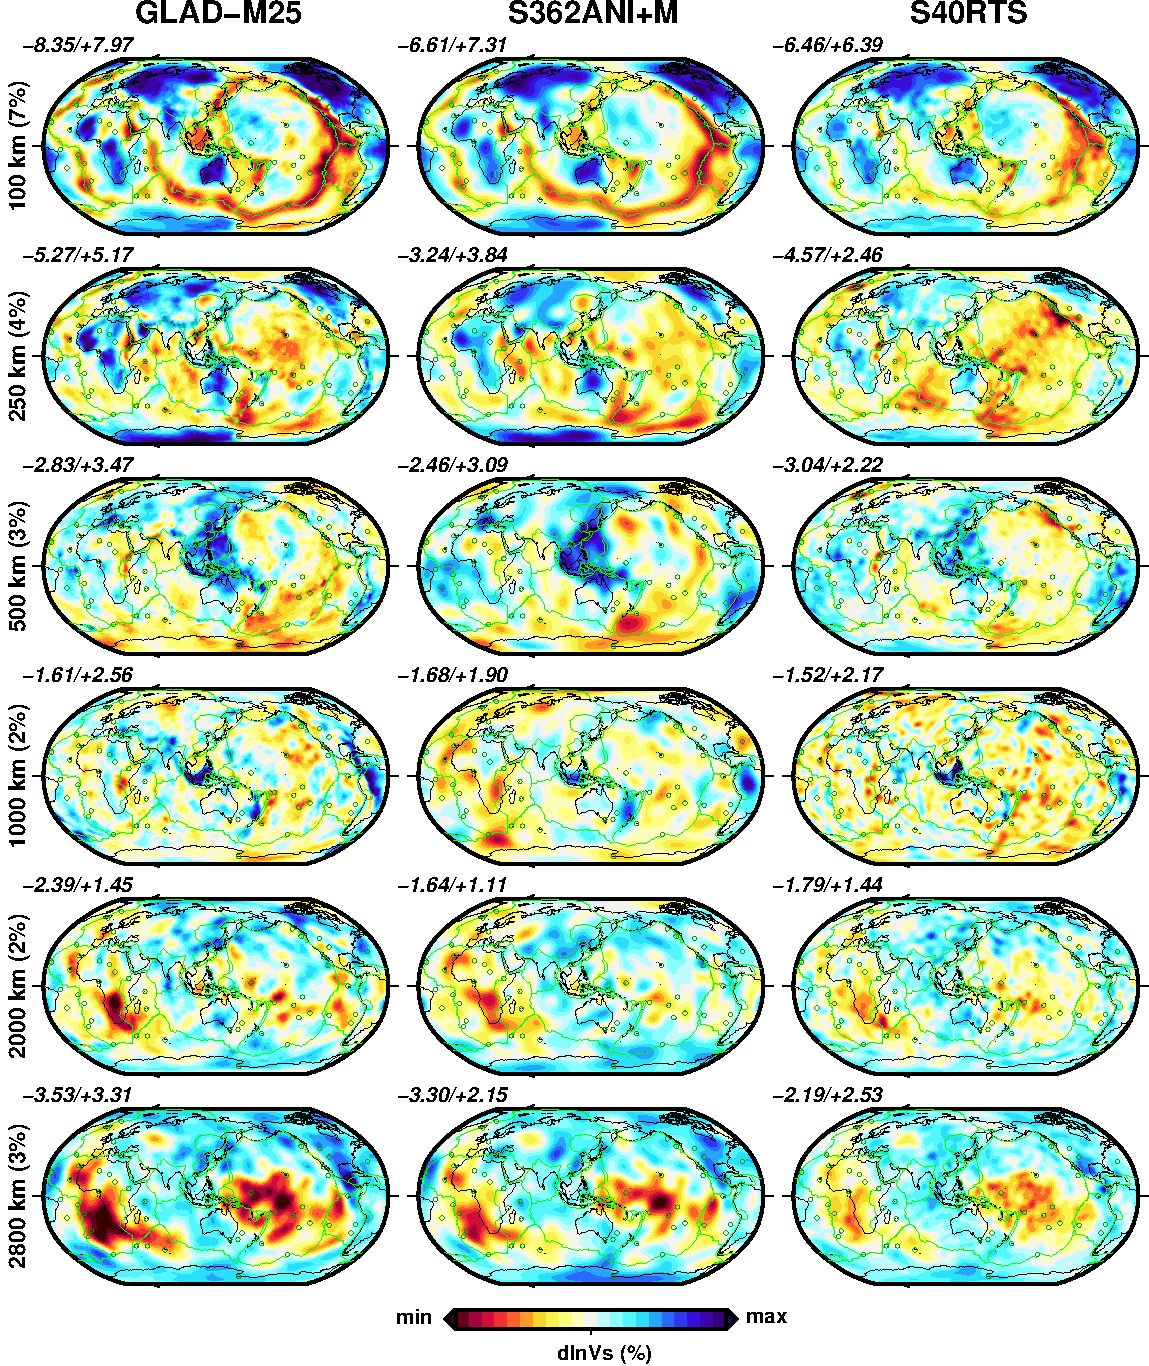
\includegraphics[width=0.9\textwidth]{figures/depth_slice/globe_vs.pdf}
  \caption{\small{Map views of global shear wavespeed perturbations at various depths for  model
  GLAD-M25~(left column), S362ANI$+$M~\citep[middle column;][]{moulik2014anisotropic},
  and S40RTS~\citep[right column;][]{ritsema2011s40rts}.
  At a given radius,
  perturbations are calculated relative to each model's average.
  The range of perturbations in shear wavespeed varies from map to map, as indicated in the top left of each panel.
  The green circles denote locations of various
  hotspots~\citep{montelli2006catalogue}.
  The range of the colorbar is the same for each row,
  and its maximum value is indicated in parentheses on the left, after
  the depth.}}
  \label{fig:global-vs}
\end{figure}

We first examine model GLAD-M25 in the context of existing global tomographic models.
In Fig.~\ref{fig:global-vs} we compare global maps of the isotropic part of our
shear wavespeed model with model S362ANI$+$M~\citep{moulik2014anisotropic},
and model S40RTS~\citep{ritsema2011s40rts}.
Overall, these models are in good agreement
at the longest wavelengths, especially GLAD-M25 and S362ANI$+$M where S362ANI$+$M is the updated version of S362ANI~\citep{s362ani}, the starting model of GLAD-M15.
The perturbations in GLAD-M25 tend to be larger than in the other models,
consistent with observations by~\cite{french2014whole,french2015broad},
whose model is also based on a form of waveform inversion.

%\begin{figure}
%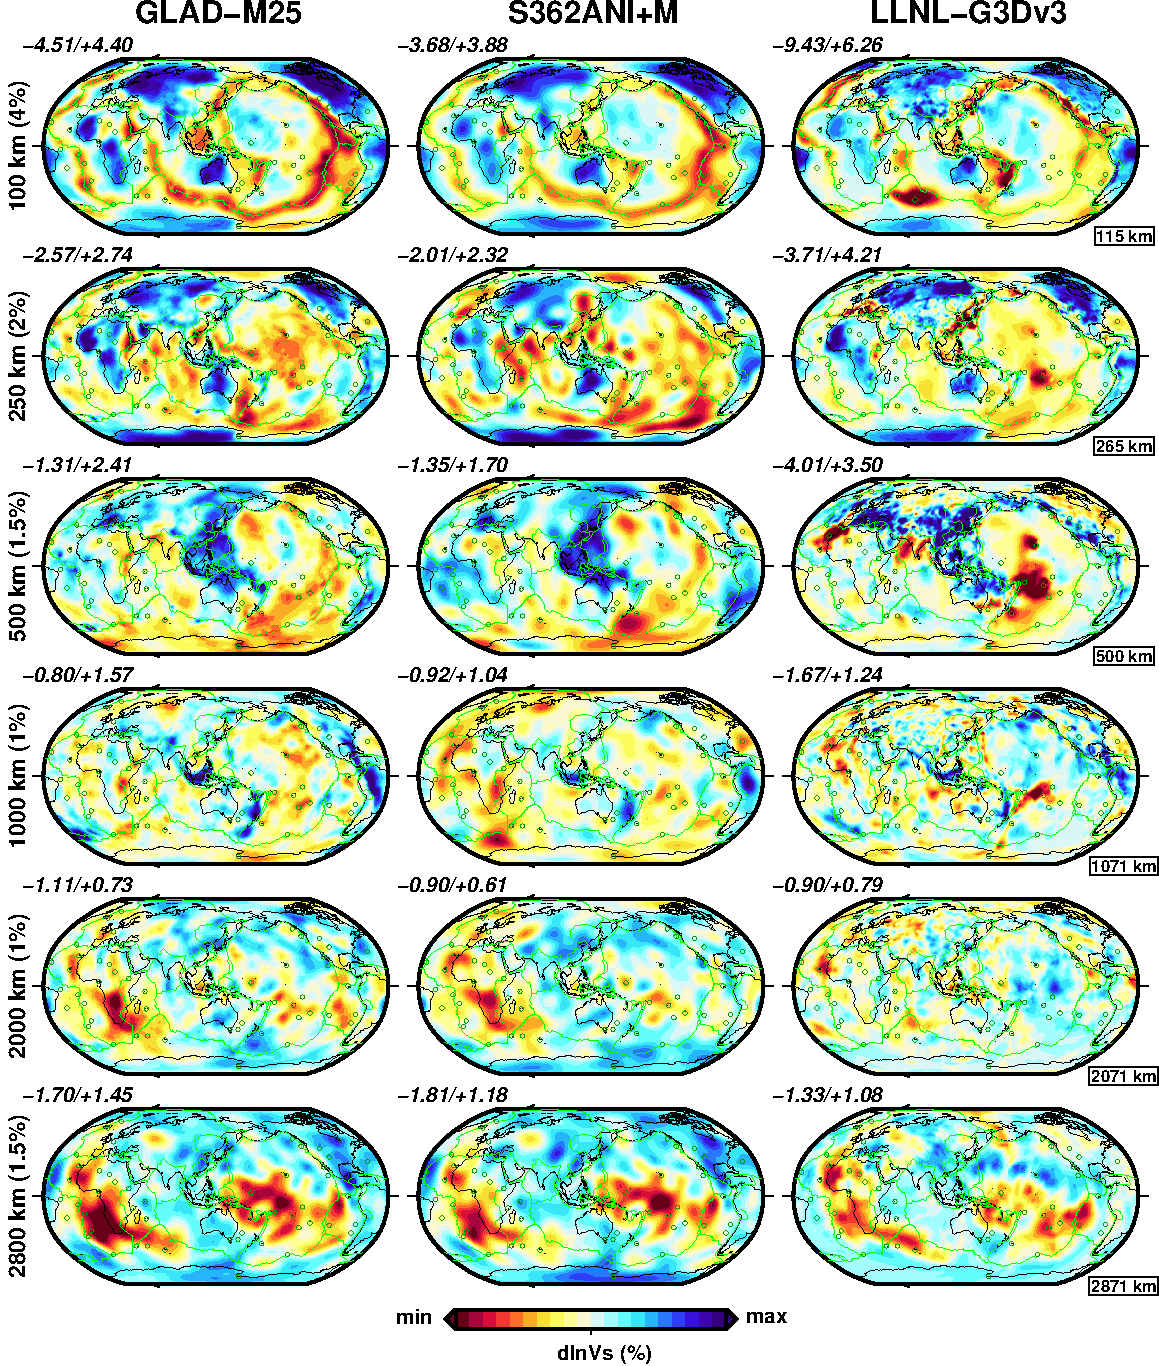
\includegraphics[width=0.9\textwidth]{figures/depth_slice/globe_vp_S362ANI-LLNL.pdf}
%  \caption{\small{Map views of global $V_\textrm{P}$ variations at various depths for our model GLAD-M25(left column), S362ANI$+$M(middle column) and LLNL-G3Dv3(right column)\citep{simmons2012llnl}. For LLNL-G3Dv3, the depths is labeled on the right bottom based on its own mesh spacing. Other plotting conventions are used similar as in Figure \ref{fig:global-vs}.}}
%\label{fig:global-vp}
%\centering
%\end{figure

An important aspect of our inversion is that it constrains shear and
compressional waves simultaneously. In Fig.~\ref{fig:global-vp} we
compare global maps of our compressional wavespeed model with global P-wavespeed models
LLNL-G3Dv3~\citep{simmons2012llnl} and GAP-P4~\citep{fukao2013subducted}.
At a depth of 100~km,
GLAD-M25 shows mid-oceanic ridges, cooling of the Pacific lithosphere,
and the roots of numerous continental cratons. In the upper mantle, LLNL-G3Dv3
exhibits the largest lateral variations,
e.g., very slow compressional wavespeeds at 500~km depth below Hawaii, Samoa, and Tahiti.
In the midmantle we can see remnants of subduction beneath South America, Indonesia,
and Tonga-Kermadec.
In the deep mantle, LLNL-G3Dv3 and GAP-P4 begin to fade out, but the long-wavelength patterns,
in particular the lowerparts of the Africa and Pacific superplumes, are very similar.

\begin{figure}
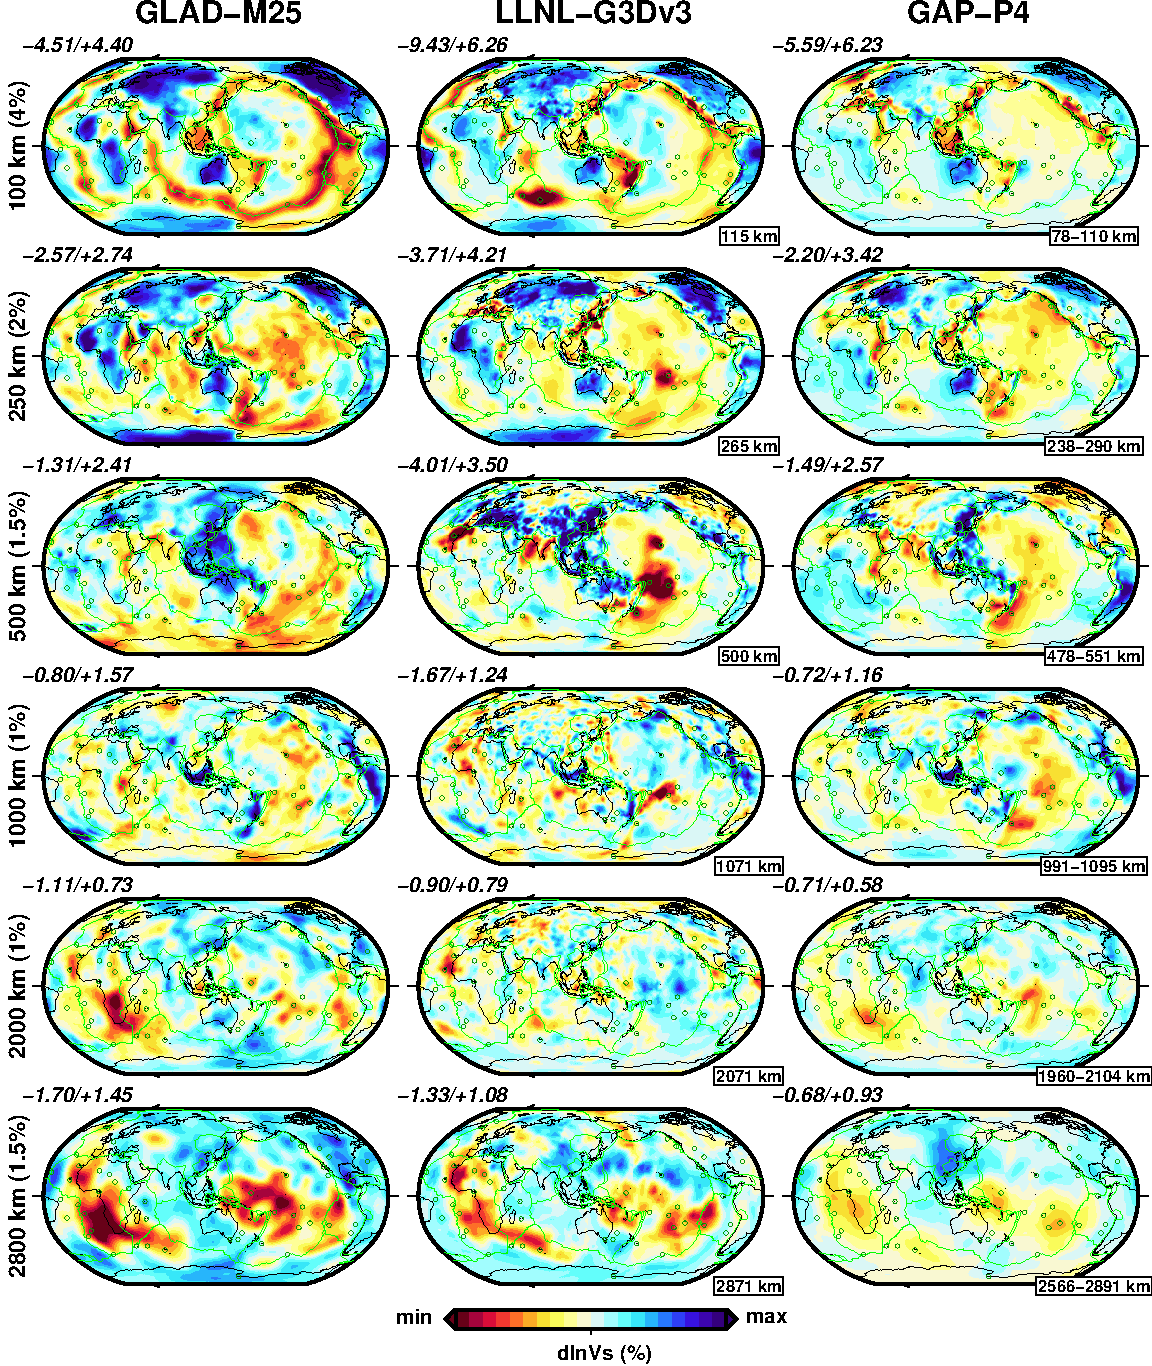
\includegraphics[width=0.9\textwidth]{figures/depth_slice/globe_vp_LLNL-GAP.pdf}
  \caption{\small{Map views of global compressional wavespeed variations at various depths for model
  GLAD-M25 (left column), LLNL-G3Dv3 \citep[middle column;][]{simmons2012llnl}, and
  GAP-P4~\citep[right column;][]{fukao2013subducted}.
  For LLNL-G3Dv3, depth ranges are labeled in the bottom right
  bottom of each panel. Other plotting conventions are as in Fig.~\ref{fig:global-vs}.}}
\label{fig:global-vp}
\centering
\end{figure}

\subsubsection{North America}

\begin{figure}
\centering
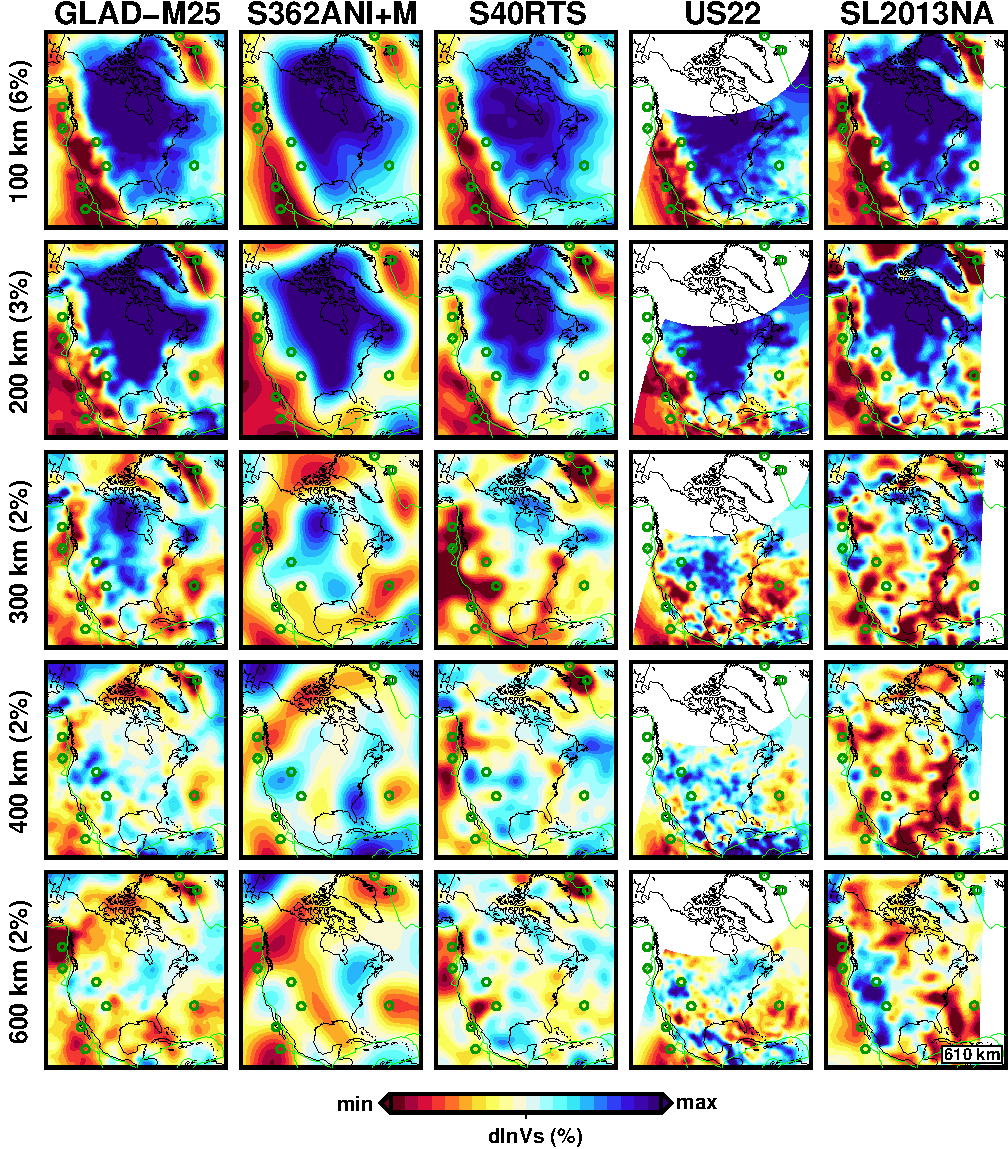
\includegraphics[width=0.9\textwidth]{figures/depth_slice/america_vs.pdf}
  \caption{\small{Map views of isotropic shear wavespeed variations beneath North America 
  for model GLAD-M25 (first column) and several global (S362ANI$+$M and S40RTS)
  and regional~\citep[US22;][]{zhu2017radial} and~\citep[SL2013NA;][]{schaeffer2014imaging}
  models. Green circles denote the locations of hotspots. For SL2013NA, we
  show a depth of 610~km instead of 600~km, reflecting its model parametrization.}}
\label{fig:america-vs}
\end{figure}

The deployment of USArray has dramatically increased data coverage across the
continental United States,
and yet despite this tremendous increase in data coverage, there is not as much agreement between different models as one might anticipate.
In this section, we compare GLAD-M25 in this region 
with two global models, S362ANI$+$M and S40RTS, and two regional models,
US22~\citep{zhu2017radial} and SL2013NA~\citep{schaeffer2014imaging}.
US22 is a radially anisotropic model based on adjoint tomography using
USArray data from 180 regional earthquakes using 15--50~s
body waves and 25--150~s surface waves.
SL2013NA is a global upper-mantle shear wavespeed model based on multimode
surface waveform tomography primarily focused on North America.

North America is characterized by a large, high-wavespeed lithospheric craton,
bounded by the Rocky Mountain Front to the West and continental
margin to the East~\citep{grand1984upper, whitmeyer2007tectonic},
with sharp tectonic boundaries
~\citep{masters1996shear, grand1997high, megnin2000three, gu2001models}.

At a depth of 100~km, we observe that the edges of the craton are sharper in
GLAD-M25 than in the other two global models,
and quite similar in shape and sharpness to the two regional models.
We can see impressions of the Snake River Plain (with Yellowstone)
and the Raton hotspot, which also have slow expressions at depths of 200~km. The PSF test we performed in this region~(Fig.~\ref{fig:psf_yellowstone})~gives us confidence on the resolution of the observed anomalies. It is also promising to see the convergence of our global model to the resolution of continental-scale studies specifically in densely covered regions.
The core of the craton exhibits fast wavespeeds at depths reaching 300~km Northwest of
Hudson Bay.
In the regional models the craton has basically faded away at these depths.
The Wyoming and Medicine Hat Blocks show a very strong and thick lithospheric
root from shallow depths to $\sim$400~km, similar to US22 but
difficult to discern in SL2013NA, which may be due to the similar theory and measurement techniques that were used in the construction of GLAD-M25 and US22.
Similar observations can be made for the Yavapai and
Mazatzal Blocks, which define the southern boundary of the large craton
~\citep{schaeffer2014imaging}.

In the 200--400~km depth range, we observe a low wavespeed anomaly beneath the Arctic
and high shear-wavespeed
anomaly within the Gulf of Mexico, which coincides spatially with the deepest
bathymetry and corresponds to a portion of ancient oceanic
lithosphere~\citep{muller2008, schaeffer2014imaging}.
A remnant of the Juan de Fuca plate,
with a high wavespeed footprint, is visible at depths of 300~km and 400~km,
where SL2013NA shows a much stronger anomaly.

In the North, we see a high wavespeed craton beneath Greenland which is partly
separated from the North American craton by low wavespeed structures beneath
Baffin Bay and the Labrador Sea, where the North American craton nicely follows
the coastline~\citep{chalmers2001development}.
In the Northeast corner of the maps we see that the Iceland hotspot is very
prominent in GLAD-M25 in all depth ranges, similar to S40RTS but largely missing
in S362ANI$+$M. In the Northwest we see a clear imprint of the Aleutian
subduction zone in the 200--400~km depth range, comparable to SL2013NA but absent
in the other global models.

In the East, at 100~km depth,
we see ageing of the Atlantic lithosphere, comparable to the other global models
~\citep{muller2008, schaeffer2014imaging}.
All models show fast anomalies beneath Newfoundland and Nova Scotia extending to
depths of 300~km.
The Bermuda hotspot has a distinct slow wavespeed impression,
getting sharper and stronger at depths of 200~km and 300~km (note differences in
the scales of the maps).
The Caribbean slab, a relatively young subduction zone, is clearly
visible in our model in the 200--400~km depth range.
At greater depths,
GLAD-M25 shows a very distinct image of the Farallon slab.

\subsubsection{Europe}

\begin{figure}[ht!]
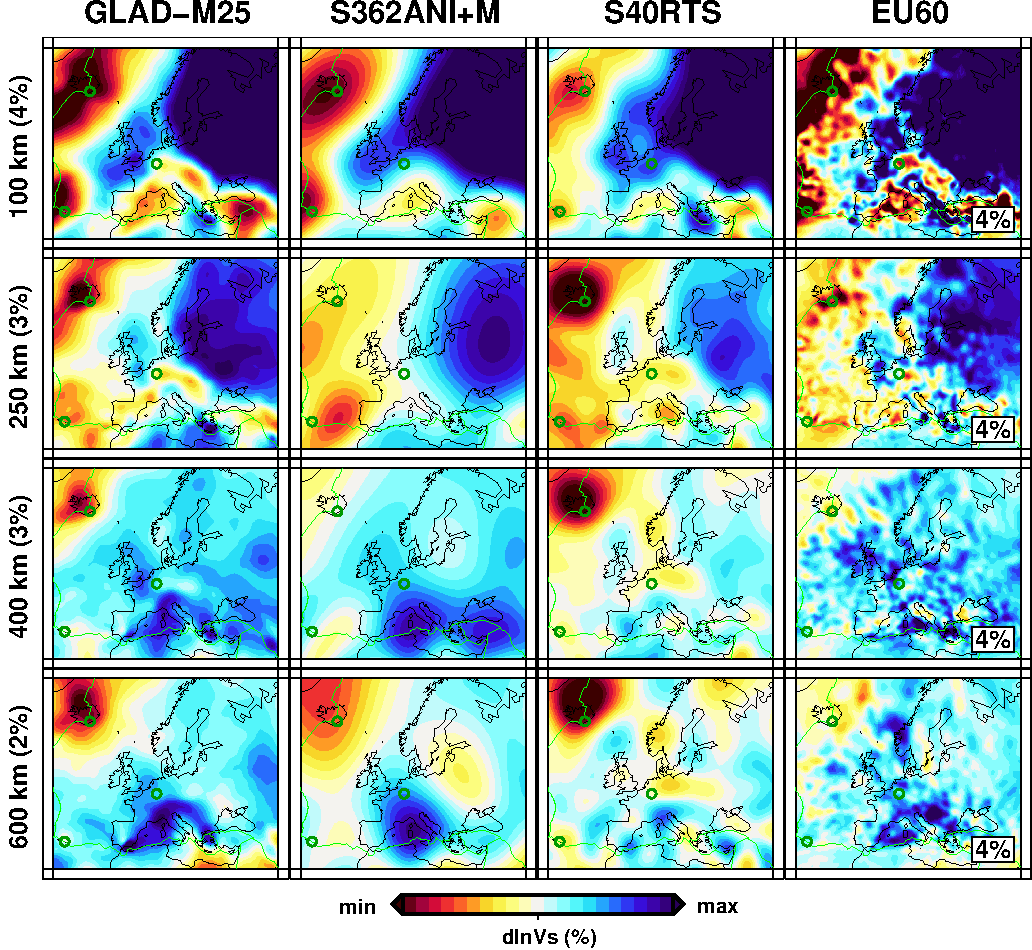
\includegraphics[width=0.9\textwidth]{figures/depth_slice/europe_vs.pdf}
  \caption{\small{Map views of isotropic shear wavespeed variations beneath Europe for model GLAD-M25 (first column), two global model (S362ANI$+$M and S40RTS), and
  one regional model~\citep[EU60;][]{zhu2015seismic}. For EU60, the range of the color
  bar is 4\% at all depths, as indicated in the bottom right bottom of the panels.}}
\label{fig:europe-vs}
\centering
\end{figure}

Fig.~\ref{fig:europe-vs} shows isotropic shear wavespeed perturbations beneath Europe.
In addition to models GLAD-M25, S362ANI$+$M, and S40RTS, we included regional
model EU60~\citep{zhu2015seismic} for comparison.
EU60 is the result of adjoint tomography of the crust and upper mantle
beneath the European continent and the North Atlantic based on the assimilation of data from
190 earthquakes recorded by 745 seismographic stations.

A defining tectonic feature of Europe is the Trans-European Suture Zone~(TESZ),
also known as the Tornquist-Teisseyre Zone,
separating the Precambrian East European Craton~(EEC) in the Northeast from
Phanerozoic Europe in the Southwest~\citep{zielhuis1994deep}.
The TESZ is very consistent across all models,
even though is much sharper in GLAD-M25 and EU60.

At depths of 100---250~km we observe high wavespeeds beneath the Central Graben
in the North Sea, which is clearly separated from the EEC.
The tectonic history of the Mediterranean is complex,
involving several regional plates and multiple past and present subduction zones
~\citep{dewey1989kinematics}.
We see slab ponding in the transition zone beneath the western Mediterranean
associated with slab roll-back of the Appennines-Maghrebides subduction zone
~\citep{wortel2000subduction, zhu2012structure}.
At shallower depths, we see low wavespeeds along its western border,
which are interpreted as back-arc extension associated with  roll-back.
Compared to S362ANI$+$M and S40RTS,
our model shows much sharper features for these tectonic structures.

In the Eastern Mediterranean, there is a distinct fast anomaly beneath the 
Dinarides Mountains, separating the Adria plate from the Pannonian Basin,
indicating subduction of the Adria plate beneath the Eurasian plate.
This anomaly gets sharper at 600~km depth.
Its southern part interacts with the Hellenic slab, which penetrates the mantle
transition zone and extends below 1,000~km in our model.
The Pannonian Basin is characterized by a low wavespeed
anomaly at depths from 100~km to 250~km.
In this depth range we also see slow wavespeeds beneath Anatolia,
stronger than in the two other global models.

In Central Europe we note the Cenozoic Ridge System~\citep{ziegler1992european},
characterized by low 
wavespeeds from the Massif Central to the Eifel. Both EU60 and
GLAD-M25 exhibit a slow anomaly beneath the northern part of the Rhine Graben,
which is interpreted as the reservoir that fuels the Eifel hotspot
~\citep{goes1999lower, zhu2015seismic}.

Beneath the Atlantic Ocean, our model enhances slow anomalies beneath the
ridges, especially underneath Iceland and the Azores.
Compared to S362ANI$+$M, Iceland becomes much stronger in the upper mantle at
depths from 250~km to 400~km, extending all the way to the mantle-transition zone.
The Azores represent a much shallower hotspot, with a maximum depth of about 250~km.

\subsubsection{Asia}

\begin{figure}[ht!]
  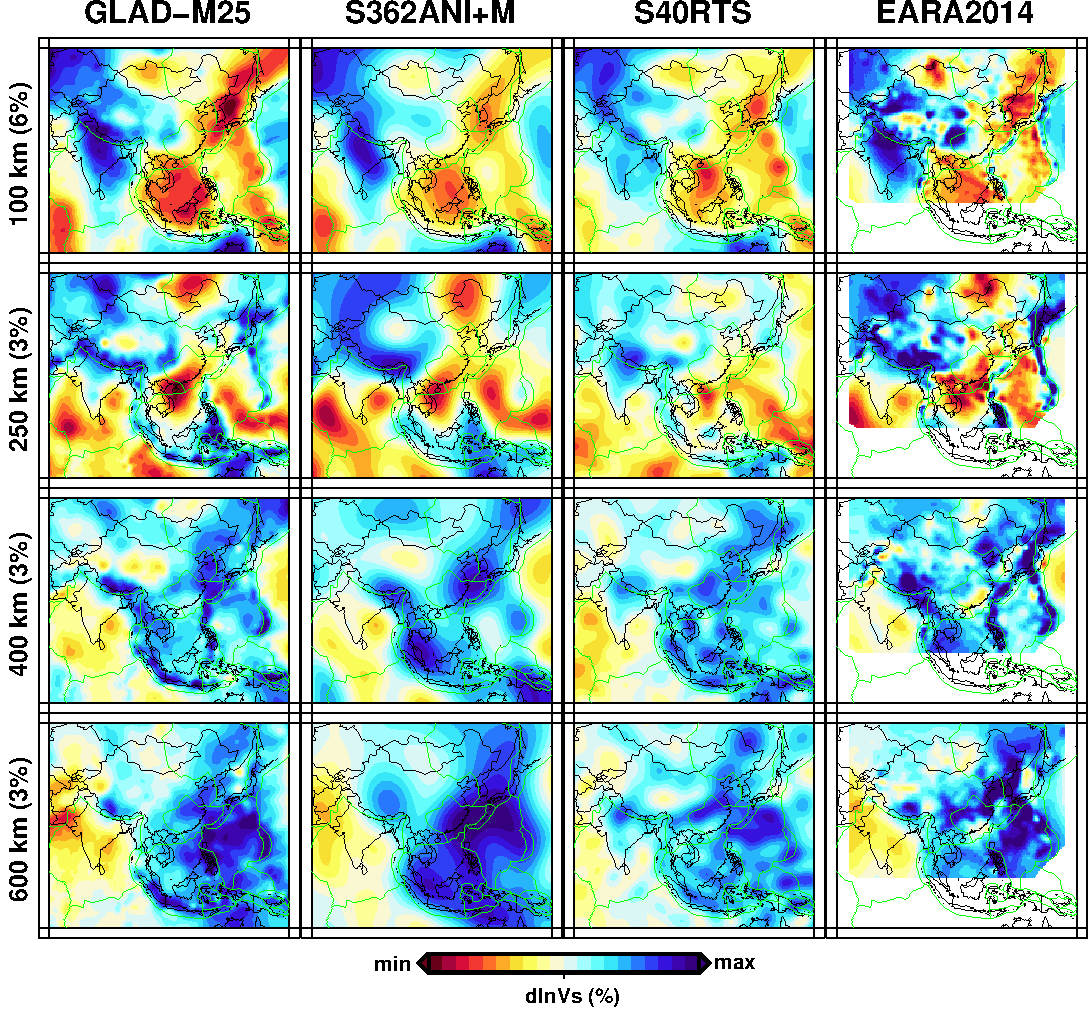
\includegraphics[width=0.9\textwidth]{figures/depth_slice/asia_vs.pdf}
  \caption{\small{Map views of shear wavespeed variations beneath Asia for GLAD-M25~(first column),
  global models S362ANI$+$M (second column) and SL2013sv (third column), and regional model EARA2014~\citep[last column;][]{chen2015multiparameter}.}}
  \label{fig:asia-vs}
  \centering
\end{figure}

Asia, like Europe, has a complex tectonic history, involving
interactions among the Indian, Eurasian, Australian, Pacific, and Philippine
plates.
Map views of GLAD-M25 centered on Asia are plotted in Fig.~\ref{fig:asia-vs},
together with S362ANI$+$M, SL2013sv~\citep{SchaefferLebedev13}, and regional model EARA2014~\citep{chen2015multiparameter}.
EARA2014 is a transversely isotropic model based on adjoint
tomography, assimilating 1.7~million frequency-dependent traveltime
measurements from 227 earthquakes recorded by 1,869 seismographic  stations.
It has superior data coverage, mainly by incorporating data from the China Array.

The Southwestern part of China is dominated by the Himalayas,
expressing the collision between India and Eurasia~\citep{lebedev2003upper}.
GLAD-M25 exhibits strong high wavespeed anomalies in this area,
which extend all the way from 100~km to 600~km, narrowing and sharpening with depth,
in good agreement with EARA2014.
The Tibetan plateau shows relatively low wavespeeds
compared to its surroundings, including the Himalayas to its South and
the Tianshan Mountains to its North, consistent with the other global
and regional studies.

The southern part of Asia shows major tectonic activity between the
Philippine, Eurasian, and Australia plates.
The Sunda trench is visible as a distinct high wavespeed anomaly below 200~km,
nicely following the plate boundary.
This feature remains very sharp at 600~km and extends
down to 1000~km.
The Manila and Philippine trenches are also much sharper in our model between 200~km and
600~km than in the other global models, and comparable to EARA2014.
The eastern edge of the map features a series of trenches following plate boundaries,
including Japan, Izu-Bonin, and Mariana.
These slabs are absent in the other global model,
but feature more prominently in EARA2014.
Along the northern edge we see low wavespeeds associated with the
Altai-Sayan and Baikal rift systems.
In terms of intra-plate activities,
at shallow depths we see clear low wavespeed impressions of the Hainan and Changbai volcanoes,
suggesting a lithospheric rather than deeper mantle origin~\citep{yin2000geologic}.
The Sichuan basin, a very localized high-wavespeed structure, extends below
250~km depth. At 600~km, most models shows a large region of high wavespeed
beneath the Philippine plate, indicating ponding of ancient subducted plates.

\subsubsection{South America}

\begin{figure}[ht!] 
  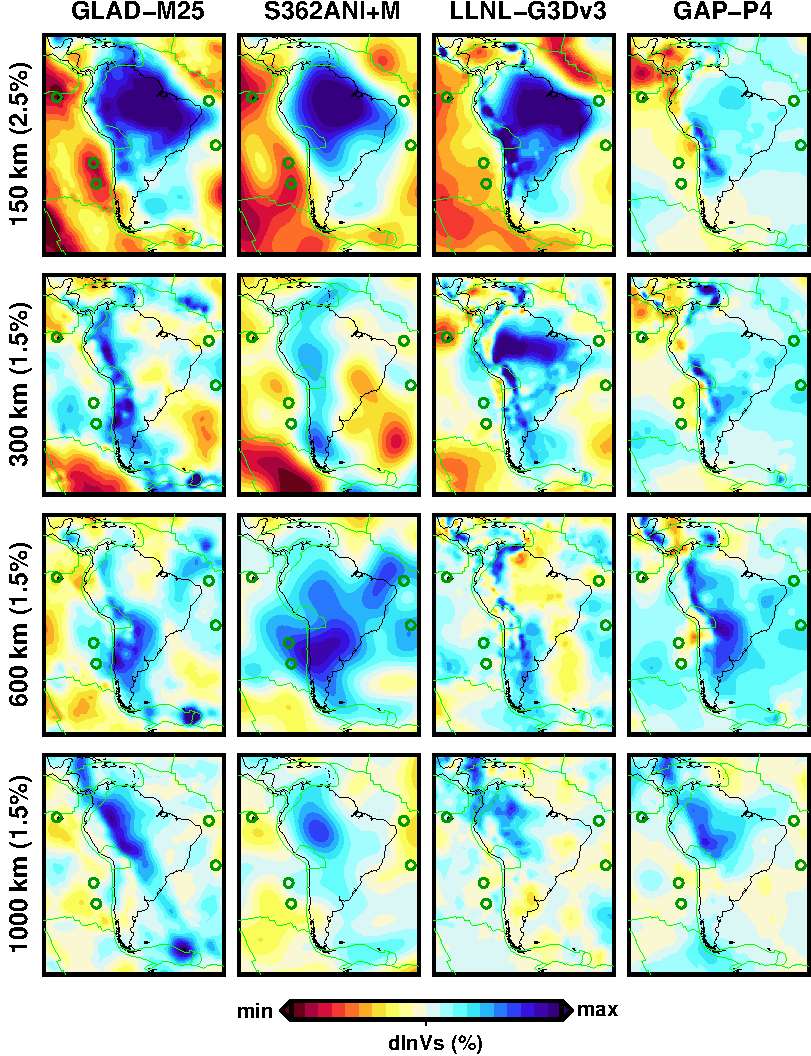
\includegraphics[width=0.9\textwidth]{figures/depth_slice/south_america_vp.pdf}
  \caption{\small{Map views of compressional wavespeed variations beneath South America for GLAD-M25~(first column) and global models S362ANI$+$M~\citep{moulik2014anisotropic} (second column), LLNL-G3Dv3~\citep{simmons2012llnl} (third column), and GAP-P4~\citep{fukao2013subducted} (fourth column).}}
  \label{fig:southamerica-vp}
  \centering
\end{figure}

Fig.~\ref{fig:southamerica-vp} shows compressional wavespeed anomalies in model GLAD-M25 in comparison with three
global models, namely, S362ANI$+$M~\citep{moulik2014anisotropic}, LLNL-G3Dv3~\citep{simmons2012llnl}, and GAP-P4~\citep{fukao2013subducted};
the latter two are $V_\textrm{P}$ models.

At 150~km depth, the northern half of South America is covered by a large lithospheric craton, exhibiting fast anomalies in all models except GAP-P4.
The Galapagos,
San Felix, and Juan Fernandez hotspots are associated with distinct low wavespeed anomalies in GLAD-M25,
but not in the other models.
At 300~km depth, we see sharpened subduction of the Nazca plate
in GLAD-M25 compared to S362ANI+M, similar in shape to model LLNL-G3Dv3.
Moving to greater depths,
we see distinct Peru and Chile slabs in GLAD-M25,
with the Chile slab ponding in the transition zone
and the Peru slab penetrating into the lower mantle and still clearly visible at 1000km depth.
These differences in behavior are consistent with GAP-P4
\citep{fukao2013subducted}.

In the south,
Scotia Arc subduction is very distinct in GLAD-M25 at all depths,
but barely observable in other models.
This is probably a consequence of coverage provided by events in the region.
To the north,
Caribbean subduction is clearly discernible in model GLAD-M25 and the two $V_\textrm{P}$ models.


\begin{acknowledgments}
This research used resources of the Oak Ridge Leadership Computing Facility,
which is a DOE Office of Science User Facility supported under contract DE-AC05-00OR22725.
Additional computational resources were provided by the Princeton Institute
for Computational Science \& Engineering (PICSciE).
We acknowledge IRIS ({\tt iris.edu}) and ORFEUS ({\tt orfeus-eu.org}) for
providing the data used in this study.
We thank Ryan Modrak, Ridvan \"{O}rsvuran, Frederik J.\ Simons, and James Smith for fruitful discussions,
and Caio Ciardelli for implementing the spherical harmonic model expansion.
The open source spectral-element software package SPECFEM3D\_GLOBE and
the seismic measurement software package FLEXWIN used for this article are
 freely available via the Computational Infrastructure for Geodynamics
 (CIG; {\tt geodynamics.org}).
 This research was supported by NSF grant~1644826.
\end{acknowledgments}

% %%%%%%%%%%%%%%%%%%%%%%%%%%%
\newpage
\bibliographystyle{gji}
\bibliography{ref.bib}

\end{document}
